\documentclass[11pt]{article}
\usepackage[margin=1in]{geometry}
\usepackage{amsmath,amssymb}
\usepackage{graphicx}
\usepackage{booktabs}
\usepackage{array}
\usepackage[colorlinks=true,linkcolor=blue,citecolor=blue,urlcolor=blue]{hyperref}
\usepackage{natbib}

\newcommand{\Msun}{M_\odot}
\newcommand{\dd}{\mathrm{d}}
\emergencystretch=3em

\title{Late-Time Mass Inflation in Double-Null Evolutions:\\
Event-Horizon-Regular Data, the Interior Linear Response\\
and Exact Integration Along a Ray}
\author{Gracen Ownby}
\date{}

\begin{document}
\maketitle

\begin{abstract}
Mass inflation at an inner horizon is a late-time phenomenon: the mass grows like $e^{\kappa_-v}$ and a double-null evolution reaches only $v\sim10^{2}$ to $3\times10^{2}$, with a truncation error that itself grows with $v$. We develop and test a method for this regime in a system where the answer can be cross-checked, the spherical Einstein--nonlinear-electrodynamics--massless-scalar system with an additive closure $M=\mu+M_N(r)$ whose static interior is a Hayward-type regular black hole ($r_-=1.057475$, $r_+=9.897927$, $\kappa_-=0.795649$, $\kappa_+=0.048969$). (1) With data regular on the event horizon, the metric exponent at the Cauchy horizon follows the surface gravity of the accumulated mass, $\kappa_-(\mu_f)$, not the static one ($0.02$--$0.08\%$ on one ray, $0.10$--$0.32\%$ on another, for $k=3/2$; $0.3$--$2.5\%$ for $k=1/2$, not relaxed). (2) The ingoing flux at the Cauchy horizon is the linear response of the static interior to the horizon flux: its kernel follows from the interior wave equation (known ingredients; the zero-frequency gain $(1+r_+^2/r_-^2)/2$ is Ori's coefficient), has decay rate $\kappa_+$, and reproduces the measured flux to $4\times10^{-4}$ at $B=0.003$; at $B=0.003$, $k=3/2$ the agreement is $3\times10^{-4}$ and constant to $2\times10^{-5}$ for $150\le v\le420$. At $B=0.03$ the flux is $3.5\%$ above the linear response of the static hole and $0.6$--$0.7\%$ ($k\ge3/2$) to $1.9\%$ ($k=1/2$) above that of the hole of the accumulated mass; the remainder is of second order in the amplitude, its coefficient depends on the profile and the injection time ($0.25$ to $6\,\mu_f$ for compact pulses), and it is bounded by $\lesssim6\,\mu_f$ over all profiles tested; there is no universal matching factor. (3) The field equations integrate exactly along a ray, $d\ln M/dv=4\pi r\phi_v^2/\rho$ for $M\gg r$, with $\rho$ the exponentially filtered flux. This reproduces the Romberg-extrapolated PDE mass to $6\times10^{-5}$ ($k=3/2$) and $2\times10^{-6}$ ($k=1/2$) over seventeen to nineteen decades of growth up to $v=108$ and is grid-converged to $10^{-5}$ in $\ln M$, whereas the grid-extrapolated PDE mass is not (the second-order error of $r_v$ grows with $v$ and its level spread understates its error by two to three orders of magnitude). A PDE reference that replaces the evolved $r_U$ and $r_v$ by the two Raychaudhuri constraints, with $y$ from a positive integral and so without calibration, agrees with the ray integration in $\ln M$ to $3\times10^{-7}$ ($B=0.03$) and $2\times10^{-6}$ ($B=0.003$) up to $v=280$, where $M\sim e^{170}$. (4) In a model driven by the kernel flux beyond $v=250$, the ray integration reaches the Ori tail law in $M$ at $v\gtrsim10^3$: $(\kappa_--d\ln M/dv)(v+1)=5.02$ for $k=3/2$ against $2k+2=5$ at $v=2500$, and $3.01$ against $3$ for $k=1/2$ at $B=0.003$. In the window reached by the PDE ($v\lesssim110$) the rate is not the tail law; for steep tails it is close to $\kappa_-(\mu_f)-2\kappa_+$ at $v\approx60$. We state what the method does not show: the closure is additive, the amplitude of $M$ is that of the discrete solution, the flux beyond $v\approx250$ at $B=0.03$ is a linear-response model, and nothing here addresses extendibility.
\end{abstract}

\section{Introduction}
\label{sec:intro}

The growth of the Misner--Sharp mass at the Cauchy horizon of a charged black hole (mass inflation; \citealt{PoissonIsrael1990,Ori1991}) is predicted by a thin-shell model whose late-time rate is $\kappa_--(2k+2)/v$ for an ingoing tail $\phi\propto v^{-k}$ \citep{Ori1991,Ori1998}. A double-null evolution of the full system can in principle test this, but the quantity of interest grows by $e^{170}$ before the grid ends, the truncation error of $r_v$ grows with it, and the prescription of the initial data on interior rays fixes the time variable to the static advanced time, in which the metric exponent is $-\kappa_-^{\rm static}$ by construction. This paper is the methodology that Paper~E \citep{PaperE} used to read the Ori law and the metric exponent from such an evolution. It is a self-contained treatment because it does not depend on the Hayward series: it applies to any spherical Einstein--scalar system with an inner horizon, and the examples are in the additive-closure system of Paper~E, where it was developed.

\paragraph{What is done.}
\begin{enumerate}
\item Data regular on the event horizon (teleological horizon data, Eddington--Finkelstein gauge), with a five-grid streaming Richardson--Romberg extrapolation of the signed series (Section~\ref{sec:ehdata}).
\item An analysis of where the ingoing flux at the Cauchy horizon comes from: the linear response of the static interior to the horizon flux, with a kernel computed from the interior wave equation (Section~\ref{sec:kernel}), tests against the evolution, its limits, and its use in a shell model.
\item The exact ray equations, their use as a reference for the extrapolated mass, and a constraint-projected PDE mass that does not rest on the evolved first derivatives (Section~\ref{sec:ray}).
\item An extension of the mass to $v=3000$ driven by the kernel flux beyond the grid, with the Ori tail law as its output (Section~\ref{sec:ray}).
\end{enumerate}

\paragraph{What comes from the literature.} The zero-frequency gain of the kernel is Ori's coefficient \citep{Ori1998}; the tail $\phi_v\propto v^{-k}$ on the event horizon with $k=2,3$ is Price's law \citep{Price1972,GundlachPricePullin1994}; the diamond scheme is that of scalar collapse \citep{GundlachPricePullin1994}; the nonlinear stability statements for charged and Kerr interiors that frame the problem are \citet{Dafermos2005,LukOh2017,HintzVasy2017,CostaFranzen2017,KehleShlapentokhRothman2019}, which we use at the level of context. What we do not find in the sources we read is the combination of the three steps above as a validated pipeline with stated error constants; that is the contribution, and it is a methodological one.

\paragraph{What this paper does not do.} It does not treat the mass-tracking closure of the series (Paper~F studies that closure's ray equations in quasi-topological gravity), the Hawking flux (Paper~E, anomaly-term model) or extendibility. Each statement below is of one of the kinds listed in the scope map of the bundle (\texttt{PAPER\_SCOPE\_MAP.md}): \emph{derived} and checked independently; \emph{reproduced} from the literature; \emph{measured} with a stated convergence statement; or \emph{model-driven}.


\section{System, closure and scheme (as in Paper~E)}
\label{sec:nlsetup}

With $ds^2=-W\,du\,dv+r^2d\Omega^2$, $W=e^{\sigma}$, and the NED monopole stress tensor ($T_{uu}=T_{vv}=0$, $\rho=\rho(r)$, $p_r=-\rho$, $p_t=-\rho-r\rho'/2$) written through $M_N(r)=m_Nr^3/(r^3+a_N)$, $\rho=M_N'/(4\pi r^2)$, and a minimally coupled massless scalar with $\mathcal L=-\tfrac12(\partial\phi)^2$, i.e.\ $T_{ab}=\partial_a\phi\partial_b\phi-\tfrac12g_{ab}(\partial\phi)^2$, the field equations are
\begin{align}
r_{uv}&=-\frac{r_ur_v}{r}-\frac{W}{4r}\bigl(1-2M_N'(r)\bigr), \label{eq:dn1}\\
\sigma_{uv}&=-\frac{2r_{uv}}{r}-8\pi\phi_u\phi_v+\frac{W\,M_N''(r)}{2r},\label{eq:dn2}\\
\phi_{uv}&=-\frac{r_u\phi_v+r_v\phi_u}{r},\label{eq:dn3}
\end{align}
with the Misner--Sharp mass and the constraints
\begin{equation}
M=\tfrac r2\bigl(1+4r_ur_v/W\bigr),\qquad r_{uu}-\sigma_ur_u+4\pi r\phi_u^2=0\quad(\text{and }u\leftrightarrow v).
\end{equation} We derived \eqref{eq:dn1}--\eqref{eq:dn3} by hand and check them in \texttt{code/eh\_init/check\_field\_equations.py}: fields with prescribed second derivatives (finite-difference Riemann tensor of the four-dimensional metric, scalar plus NED-monopole stress tensor) obey $G_{ab}-8\pi T_{ab}=0$ in all four components to $3\times10^{-6}$ when \eqref{eq:dn1}, \eqref{eq:dn2} and the constraints are imposed, and each component departs by $0.07$--$1.6$ when its own second derivative is changed by $0.1$; $\Box\phi=0$ is \eqref{eq:dn3} to $10^{-15}$. The static Hayward interior is reproduced by the $A=B=0$ validation below. The closure is \emph{additive}, $M=\mu+M_N(r)$, where $\mu$ is the part of the mass carried by the scalar: $G=(\partial_rM)_m=M_N'(r)$ is independent of $M$, as in the Reissner--Nordstr\"om case; Paper~E shows (under stated assumptions) why this is the only closure a separately conserved dark sector allows. It is not the mass-tracking closure of this series ($a\propto m$): $a_N$ and $m_N$ are fixed by the NED charge, and the static sector of the mass-tracking closure is realised in four-dimensional quasi-topological gravity, whose dynamics differ from this system (Paper~F). The runs below therefore test a method, in a Lagrangian system with known ingredients; they do not test the $s=0$ metric of the series. We use $m_N=5$, $a_N=10$ (so $\ell^2=a_N/2m_N=1$), for which the static interior has $r_-=1.057475$, $r_+=9.897927$, $\kappa_-=0.795649$, $\kappa_+=0.048969$.

\paragraph{Scheme.} The evolved variables are $r,\sigma,r_u,r_v,\sigma_u,\sigma_v,\phi_u,\phi_v$ (first-order form), so that quantities that are exponentially small near the Cauchy horizon, such as $r_u$, $r_v$ and $W$, keep full relative precision. The scheme is a double-null diamond scheme of the type used for scalar-field collapse \citep{GundlachPricePullin1994}, extended by evolving the first derivatives as independent variables: $r,\sigma$ are advanced by the diamond identity and the first derivatives by trapezoidal integration along the characteristic edges, with three predictor-corrector sweeps. Initial data on $v=0$ and on $u=-6$: $\sigma$ is set to its static value on both rays, $r$ follows from the Raychaudhuri constraint, $\phi=B+A\,e^{-u^2}$ on $v=0$ and $\phi=B(1+v)^{-k}$ on $u=-6$, $B=A/10$, $k=3/2$ unless stated. Prescribing $\sigma$ fixes the advanced time $v$ on the initial rays to be the static advanced time of the background, which is also the time in which the Ori tail is written; this matters for the interpretation below. The other natural prescription, fixing $r(v)$ to its static value and letting $\sigma$ follow from the constraint, forces $\sigma_v\sim e^{\kappa_-v}v^{-5}$ along the tail, so that $W$ underflows; it is a different, badly behaved data set, not a different physics, and is not used.

\paragraph{Validation.} For $A=B=0$ the code reproduces the static interior with error $1.1\times10^{-3},\,2.8\times10^{-4},\,6.9\times10^{-5},\,1.7\times10^{-5}$ at $h=0.08,\dots,0.01$ (measured order $1.998$--$2.000$). With a pulse, the $L_2$-norm of the relative Raychaudhuri residual in the $u$ direction is $2.2\times10^{-3},\,5.4\times10^{-4},\,1.4\times10^{-4}$ for $v\le20$ and $5.3\times10^{-3},\,1.3\times10^{-3},\,3.3\times10^{-4}$ for $20<v\le60$ at $h=0.08,0.04,0.02$ (order $2.00$); in the $v$ direction it is $1.2\times10^{-3},\,2.9\times10^{-4},\,7.3\times10^{-5}$ for $v\le20$ (and $3.4\times10^{-4},\,8.4\times10^{-5},\,2.1\times10^{-5}$ for $20<v\le58$). Grids are $u\in[-6,u_1]$, $v\in[0,v_1]$ with $h_u=h_v=h$.


\section{Data regular on the event horizon}
\label{sec:ehdata}

\paragraph{Purpose.} In the data of Section~\ref{sec:nlsetup} the function $\sigma$ is prescribed static on the initial rays, so $\sigma_v\to-\kappa_-^{\rm static}$ at the Cauchy horizon by construction. A shift of $\kappa_-$ from the mass the tail adds to the hole can only show in a time variable that is fixed on the event horizon and is the exterior advanced time. We therefore start the evolution on the event horizon.

\paragraph{Construction.} Let $U=e^{\kappa_+u}$, so that $\mathcal H^+=\{U=0\}$ and the metric is $ds^2=-\tilde W\,dU\,dv+r^2d\Omega^2$, regular there. The static solution is a function of $x=Ue^{\kappa_+v}$: $r=r_++z(x)$ with $dr/d\ln x=f(r)/2\kappa_+$ ($f=1-2M_N/r$), $\tilde W=-f/(\kappa_+U)$, $r_U=-\tilde W/2$; the interior branch ($x\ge1$) is integrated in $\ln(r-r_-)$, since $r-r_-$ is exponentially small. On $\mathcal H^+$ we impose the Eddington--Finkelstein gauge $r_U=-\tilde W/2$, which gives $\tilde\sigma_v=-r_v/r+(1-2M_N')/(2r)$, and prescribe the tail $\phi(0,v)=B(1+v)^{-k}$. The radius $r(v)$ on $\mathcal H^+$ follows from the Raychaudhuri equation $r_{vv}=\sigma_vr_v-4\pi r\phi_v^2$ with $r(0)=r_+$ and $r_v(v_{\max})=0$: the horizon is teleological and grows by $\Delta r_H\sim4\pi r\int\phi_v^2dv/\kappa_+$. Backward integration from $v_{\max}$ is the stable direction; the final radius $r_f$ is fixed by $r(0)=r_+$, and $\mu_f=r_f/2-M_N(r_f)$ is the mass parameter of the final static hole. Fixing $r_U=-\tilde W/2$ fixes $v$ up to a shift, and at late times it is the Eddington--Finkelstein time of the final hole, so $\kappa_-(\mu_f)$ is the surface gravity with respect to this $v$. The ray $v=0$ carries the static solution with $\phi=B$ and no outgoing flux, and $\phi_v$, $r_v$, $\sigma_v$ on it are integrated along $U$. A uniform grid in $U$ fails at late $v$, because the horizon transition sits at $U\sim e^{-\kappa_+v}$, a coordinate effect of $U=e^{\kappa_+u}$ (a run with $h_U=0.04$ produced NaN at $v\approx56$ and one with $h_U=0.02$ at $v\approx70$; \texttt{t\_uniform.py}). We use $U=c\,(e^{\kappa_+\varsigma}-1)/\kappa_+$, $c=0.2\,e^{-\kappa_+v_1}$, uniform in $\varsigma$, so that the grid is uniform in $U$ near $\mathcal H^+$ and logarithmic beyond, with $\sigma_\varsigma=\tilde\sigma+\ln g'$, $r_\varsigma=r_Ug'$, $\sigma_{\varsigma\varsigma}=\tilde\sigma_Ug'+\kappa_+$, $\phi_\varsigma=\phi_Ug'$. The evolution routine is the unchanged one of Section~\ref{sec:nlsetup}. For $B=0$ the evolution converges at second order to the exact static solution to $v=100$ in $\sigma$ and $\sigma_v$ (the $\sigma_v$ error at $U=1$, $v=100$ is $2.0\times10^{-2},\,5.6\times10^{-3},\,1.4\times10^{-3}$ for $h_\varsigma=h_v=0.2,0.1,0.05$); $r_U$, which is exponentially small in the interior, is not reproduced there to relative accuracy (its logarithm is off by many e-folds), because its size is set by the truncation error (below), and we do not use it. (The same holds for $y=-r_U/\tilde W$, which equals $1/2$ on the static solution: on $U=1$ the single-grid values are $-0.8,\,-3.7\times10^{3},\,-1.1\times10^{7},\,-8.7\times10^{13}$ at $v=40,\,50,\,60,\,80$ on the coarsest grid and the three-grid Romberg value is wrong by $7$ at $v=60$. With the tail the physical $y$ is much larger than this noise at $v\approx60$, which is what Section~\ref{sec:ray} uses.)

\paragraph{The exponent is dynamical ($k=3/2$).} With the tail on $\mathcal H^+$ and nothing else, $\sigma_v$ on a ray settles to $-\kappa_-(\mu_f)$, where $\kappa_-(\mu)$ is the inner surface gravity of the static hole of mass parameter $\mu$ (Table~\ref{tab:eh}; five grids, Romberg-extrapolated). The predicted shifts from the static value $0.795649$ are $1.4\%$ ($B=0.03$) and $4.0\%$ ($B=0.05$) ($2.5\%$ at $B=0.04$, where only two grids were run: Richardson value $0.77622$ against $0.775856$). On the ray $U=0.3$ at $v=95$ the extrapolated values lie $0.024\%$ and $0.077\%$ above the predictions; the single-grid values at $h=0.05$ lie $0.15\%$ and $0.21\%$ above, and the sequences converge at second order (ratios of successive differences $3.98,\,4.0,\,4.0$ for each of the three $k=3/2$, $B=0.03$, $k=1/2$, $B=0.03$ and $k=3/2$, $B=0.05$ series). The local mass parameter $\mu_{\rm loc}=M-M_N(r)$ measured before inflation sets in agrees with $\mu_f$ to $3\times10^{-4}$--$7\times10^{-4}$ on the ray $U=0.1$ for $40\le v\le65$ ($9.959\times10^{-3}$ against $9.956\times10^{-3}$ at $v=40$, $B=0.03$), and to $0.3$--$0.9\%$ on the ray $U=0.3$ of the table; this changes $\kappa_-$ by $\lesssim10^{-4}$. The shift of $\kappa_-$ from the accumulated mass is therefore a measured effect, not a gauge identity.

Two qualifications. First, for $k=1/2$ the extrapolated $|\sigma_v|$ lies $0.27\%$ ($B=0.03$) and $0.80\%$ ($B=0.05$) above the prediction on $U=0.3$ (and $0.80\%$ and $2.5\%$ on $U=1$, where the $B=0.05$ value $0.79669$ even exceeds the static $0.795649$), an order of magnitude more than for $k=3/2$ ($0.024\%$ and $0.077\%$ on $U=0.3$, $0.10\%$ and $0.32\%$ on $U=1$). The excess is not a convergence failure (the five-grid sequence converges at second order, Table~\ref{tab:eh}); it is a relaxation effect that is larger for the slower tail, whose later horizon flux still adds mass after the time of the measurement. We have not derived this, but the long runs of Section~\ref{sec:kernel-long} show the excess $|\sigma_v|-\kappa_-(\mu_f)$ falling for both tails, from $1.1\times10^{-4}$ at $v=60$ to $1.1\times10^{-5}$ at $v=290$ ($k=1/2$) and from $3.2\times10^{-5}$ to $5\times10^{-8}$ ($k=3/2$) at $B=0.003$. Second, what is measured is $\sigma_v$, not the rate of mass inflation. For every $B$ tried ($0.03,0.04,0.05$) the rays with $U>U_c(B)$ reach $r<0$ ($U_c\approx3.6,\,3.3,\,2.9$ from the first NaN column, with $\sigma\to-\infty$ there; the first-NaN $v$ depends on $h$); we have not established whether this locus is spacelike or that there is a threshold in $B$ in this range. The rays used here, $U\le1.2$, lie outside the future of that region.

\begin{table}[h]
\centering
\caption{$|\sigma_v|$ at $v=95$ for tail-only data on $\mathcal H^+$ ($v_1=110$), five grids $h_\varsigma=h_v=0.05,\dots,0.003125$ and their Romberg extrapolation; ray $U=0.3$ (and $U=1$ for the extrapolant). Prediction: $\kappa_-(\mu_f)$; static value $0.795649$.}
\label{tab:eh}
\footnotesize
\begin{tabular}{@{}ccccccccc@{}}
\toprule
$k$ & $B$ & $\mu_f$ & $\kappa_-(\mu_f)$ & $h=0.05$ & $0.0125$ & $0.003125$ & extrap.\ $U{=}0.3$ & extrap.\ $U{=}1$\\
\midrule
$3/2$ & $0.03$ & $9.956\times10^{-3}$ & $0.784821$ & $0.78597$ & $0.78507$ & $0.78502$ & $0.78501$ & $0.78561$\\
$3/2$ & $0.05$ & $2.7757\times10^{-2}$ & $0.763567$ & $0.76518$ & $0.76422$ & $0.76416$ & $0.76416$ & $0.76604$\\
$1/2$ & $0.03$ & $5.913\times10^{-3}$ & $0.789303$ & $0.79231$ & $0.79147$ & $0.79142$ & $0.79142$ & $0.79557$\\
$1/2$ & $0.05$ & $1.6461\times10^{-2}$ & $0.777349$ & $0.78443$ & $0.78364$ & $0.78359$ & $0.78358$ & $0.79669$\\
\bottomrule
\end{tabular}
\end{table}

\paragraph{The raw mass function is noise-dominated; its extrapolation is not.} With the tail alone, $M$ on the Cauchy-horizon rays is not a physical output of any single grid. For $B=0.03$, $k=3/2$, $U=1$, $v=100$, the five grids $h_\varsigma=h_v=0.05,\dots,0.003125$ give $M=-9.1\times10^{17},\,-2.6\times10^{17},\,-6.7\times10^{16},\,-1.5\times10^{16},\,-1.8\times10^{15}$ and the extrapolation $+2.5\times10^{15}$ (for $k=1/2$: finest $2.4\times10^{17}$, extrapolated $2.5\times10^{17}$; at $v=60$ the raw values are $-6\times10^{3}$ to $3.2\times10^{4}$ for $k=1/2$). The single-grid error grows with $v$: for $k=3/2$, tail only, the finest grid is off by $2\%$, $18\%$ and $171\%$ of the extrapolated $M$ at $v=60,80,100$ (the next grid by $9\%$, $71\%$, $683\%$), and the rate of the single-grid $M$ over $[84,88]$ is undefined on four of five grids ($M<0$) and $0.632$ on the finest against $0.691$ for the extrapolant ($8.5\%$ low). The errors of the single grids against the extrapolant at $v=100$ ($k=3/2$) are $9.1,\,2.7,\,0.69,\,0.17,\,0.044\times10^{17}$ and fall by successive factors $3.4,\,3.9,\,4.0,\,4.0$, approaching the factor $4$ of an $h^2$ law. The cause we propose is that the second-order truncation error of the horizon transition acts as a mass perturbation, amplified by the same blueshift as a physical one: for $B=0$ the spurious $\mu=M-M_N(r)$ at $U=0.3$, $v=40$ is $(1.5\text{--}1.7)\times10^{-3}\,(h_\varsigma^2+h_v^2)$ over five combinations of $(h_\varsigma,h_v)$ with $h_\varsigma,h_v\in[0.025,0.1]$ (\texttt{aniso.py}; the two anisotropic pairs $(0.1,0.025)$ and $(0.025,0.1)$ give $1.7$ and $1.5\times10^{-3}$); for the tail data Section~\ref{sec:ray} locates the error of the single-grid $M$ in the factor $\rho=-r_v$ and, at small $B$, in the absolute error of $y-\tfrac12$. Because the error is a series in even powers of $h$, Romberg extrapolation over the five grids removes its leading terms: the two highest Romberg levels (all five grids; the four finest) agree to $1.4\times10^{-6}$ in relative terms at $v\ge60$ on all four rays of the five main series ($1.1\times10^{-4}$ including the wide-seed run) (\texttt{report\_stream.py}), and the extrapolated $M$ is positive and increasing, as \eqref{eq:muv} requires ($\mu_v>0$ for $r_u<0$). What supports calling it converged in the window $v\lesssim110$ is this internal agreement together with the relation tested below, which the single-grid values do not satisfy; it is not an independent solution and the rate test does not fix the amplitude of $M$ (any solution with the same $\sigma_v$ and $\phi_v$ obeys it). Section~\ref{sec:ray} shows that at larger $v$, and at the smaller amplitude $B=0.003$, the level spread of $M$ understates its error by two to three orders of magnitude, and gives a PDE reference, built from the Raychaudhuri constraints, that is not subject to it.

The relation to be tested follows from the field equations. From $r_{uv}$ and the $v$-Raychaudhuri equation, with $\mu=M-M_N(r)$,
\begin{equation}
\mu_v=-8\pi r^2\,\frac{r_u}{W}\,\phi_v^2\equiv g ,\label{eq:muv}
\end{equation}
which we checked on seeded data where $M$ is accurate (ratio of the two sides $1.0016\to1.0004$ at $v=5$, $U=0.5$, and $0.994\to0.9985$ at $v=30$, $U=1$, for $h=0.05\to0.025$). If $g$ grows quasi-exponentially at the rate $\lambda=d\ln g/dv$, then $\mu\simeq g/\lambda\,(1+\lambda'/\lambda^2)$ and $d\ln\mu/dv=\lambda-\lambda'/\lambda$. For $M\gg M_N$ (so that $d\ln\mu=d\ln M$), with $r_v/r$ and $W(1-2M_N')/(4rr_u)$ negligible, $\lambda=|\sigma_v|+2\,d\ln|\phi_v|/dv$, the differential form of the Ori law. This is an asymptotic consequence of the equations, not an identity of the discrete variables ($M$, $\sigma_v$, $\phi_v$ are evolved independently), and it tests quasi-stationarity and the discretization rather than new physics. It requires $\lambda'/\lambda^2\ll1$, so it cannot hold near a node of $\phi_v$, where $g\to0$.

\paragraph{Rate against the relation.} We evolve to $v_1=110$ on five grids (streaming kernel, \texttt{stream.c}, bitwise identical to the stored-array kernel on a test run; $U\le1.5$; $h_\varsigma=h_v$), take $M$, $\sigma_v$, $\phi_v$ interpolated linearly in $\varsigma$ to the ray, and extrapolate each. Table~\ref{tab:ehrate} compares the rate of the extrapolated $M$ over $\Delta v=4$ with $\lambda$ and with $\lambda-\lambda'/\lambda$ (window averages). For the five series (tail-only $k=1/2,3/2$; seeded $k=1/2,3/2,5/2$ with $A=0.02$ at $U_0=1$, $w=0.3$, $B=0.03$) the difference between the rate and $\lambda-\lambda'/\lambda$ is $\le2\times10^{-4}$ in the windows $[72,76]$, $[84,88]$, $[96,100]$, $[104,108]$ on the rays $U=1$ and $U=1.2$, and on $U=0.6$ from $[72,76]$ ($\le2\times10^{-4}$), and, for the seeded runs on $U=1$, $+0.7$ to $+2.1\times10^{-3}$ at $[60,64]$; we do not know the cause (the seeded $\phi_v$ has a node at $v\approx44.5$--$47.5$, some fifteen units earlier). For the tail alone the agreement is $\le2\times10^{-4}$ also at $[60,64]$. The relation is valid only once the mass is large: on the rays $U=0.3$ and $0.6$ the difference is $0.01$--$0.7$ while $M\lesssim10$ (e.g.\ $-1.4\times10^{-2}$ for $M=9$, $k=3/2$, tail only, $U=0.3$, $[84,88]$) and $\le4\times10^{-4}$ once $M\gtrsim4\times10^{2}$ (all five series, all four rays, windows from $[72,76]$). A second tail amplitude, $B=0.05$ (tail only, five grids, $\kappa_-(\mu_f)=0.77735$ for $k=1/2$ and $0.76357$ for $k=3/2$), gives the same: $|\text{rate}-(\lambda-\lambda'/\lambda)|\le5\times10^{-4}$ at $[60,64]$ and $\le2\times10^{-4}$ from $[72,76]$, with rates $0.746$--$0.753$ ($k=1/2$) and $0.672$--$0.675$ ($k=3/2$); the finest-grid $M$ at $v=100$ is off by $2\%$ ($k=1/2$) and $53\%$ ($k=3/2$), less than at $B=0.03$ ($171\%$ for $k=3/2$), consistent with a truncation noise that does not grow with $B$ while the physical mass does (the noise was measured only at $B=0$); at $B=0.003$ the extrapolation of $M$ itself fails by $v\approx100$ for $k=3/2$ (Section~\ref{sec:ray}). The correction $\lambda'/\lambda$ matters: without it the difference is up to $1.5\times10^{-3}$ at $[72,76]$ (seeded $k=1/2$) and $5.8$--$7.0\times10^{-3}$ at $[60,64]$ (seeded $k=3/2,5/2$).

\begin{table}[h]
\centering
\caption{Ray $U=1$, $B=0.03$, five-grid extrapolation: rate of $M$ over $[v,v+4]$, $\lambda=|\sigma_v|+2\,d\ln|\phi_v|/dv$, $\lambda-\lambda'/\lambda$ and $|\sigma_v|$ (window averages). For comparison $\kappa_-(\mu_f)=0.78930,\,0.78482,\,0.78342$ for $k=1/2,3/2,5/2$. ``seed'' is $A=0.02$, $U_0=1$, $w=0.3$.}
\label{tab:ehrate}
\begin{tabular}{@{}lccccc@{}}
\toprule
data & window & rate & $\lambda$ & $\lambda-\lambda'/\lambda$ & $|\sigma_v|$\\
\midrule
$k=1/2$, tail only & $[60,64]$ & $0.7338$ & $0.7347$ & $0.7340$ & $0.8008$\\
 & $[84,88]$ & $0.7457$ & $0.7463$ & $0.7457$ & $0.7967$\\
 & $[104,108]$ & $0.7543$ & $0.7548$ & $0.7544$ & $0.7945$\\
$k=3/2$, tail only & $[60,64]$ & $0.6868$ & $0.6872$ & $0.6869$ & $0.7880$\\
 & $[84,88]$ & $0.6911$ & $0.6913$ & $0.6911$ & $0.7860$\\
 & $[104,108]$ & $0.6947$ & $0.6950$ & $0.6947$ & $0.7853$\\
$k=1/2$, seed & $[60,64]$ & $0.7086$ & $0.7077$ & $0.7079$ & $0.7635$\\
 & $[84,88]$ & $0.7272$ & $0.7285$ & $0.7273$ & $0.7780$\\
 & $[104,108]$ & $0.7425$ & $0.7433$ & $0.7426$ & $0.7826$\\
$k=3/2$, seed & $[60,64]$ & $0.6948$ & $0.6890$ & $0.6930$ & $0.7704$\\
 & $[84,88]$ & $0.6861$ & $0.6866$ & $0.6861$ & $0.7803$\\
 & $[104,108]$ & $0.6926$ & $0.6930$ & $0.6926$ & $0.7831$\\
$k=5/2$, seed & $[60,64]$ & $0.6958$ & $0.6889$ & $0.6938$ & $0.7701$\\
 & $[84,88]$ & $0.6808$ & $0.6811$ & $0.6808$ & $0.7794$\\
 & $[104,108]$ & $0.6838$ & $0.6840$ & $0.6838$ & $0.7819$\\
\bottomrule
\end{tabular}
\end{table}

\paragraph{Robustness to the seed.} Four further seeds were run for $k=3/2$, $B=0.03$ ($A$, $U_0$, $w$): $(0.01,1,0.3)$ on four grids, $(0.02,0.7,0.2)$ and $(0.02,1,0.5)$ on five, $(0.03,0.6,0.3)$ on four. The first agrees to $\le5\times10^{-5}$ for $v\ge72$ ($8\times10^{-4}$ at $[60,64]$). The second agrees to $5\times10^{-4}$ at $[72,76]$ and $\le5\times10^{-5}$ after; at $[60,64]$ it is off by $5.6\times10^{-3}$ ($\phi_v$ has nodes at $v\approx34$ and $54$). The third fails at late times: $\phi_v$ changes sign at $v\approx92$, the rate is $0.52,\,0.38,\,1.07,\,0.82$ over $[72,76]$, $[84,88]$, $[96,100]$, $[104,108]$ while $\lambda-\lambda'/\lambda$ is $0.52,\,0.61,\,1.09,\,0.82$; only the first and last windows are within $2\times10^{-3}$ (the differences are $-1.8\times10^{-3}$, $-0.23$, $-0.018$, $+2.0\times10^{-3}$): the relation fails over about $\pm20$ units of $v$ around the node and is off by $1.8\times10^{-3}$ and $2.0\times10^{-3}$ in the end windows. This is the failure that the derivation predicts ($g\to0$ at the node, $\lambda'/\lambda^2$ not small), not a discretization effect (the extrapolation levels agree). The fourth ($A=0.03$ at $U_0=0.6$) is not in the perturbative regime: on the analysis ray $U=1$ the solution reaches $r<0$ between $v=40$ and $60$, and on $U=0.6$ the extrapolated $M$ is $3.7\times10^{9}$ at $v=60$ and the four grids give both signs at $v=80$; we do not analyse it. The relation is therefore verified away from nodes of $\phi_v$ and for perturbative seeds, and is not claimed beyond that.

\paragraph{The ingoing flux on the rays: observations.} On these rays $|\phi_v|$ is $7$--$110$ times (tail-only and seeded $k=1/2,3/2$; $\sim3\times10^{3}$ for the seeded $k=5/2$) the tail transported from $\mathcal H^+$ with the high-frequency factor $r_+/r_-\approx9.36$; against the zero-frequency response $T(0)\,j(v)$ of Eq.~\eqref{eq:T0}, which is the proper quasi-static comparison, it is $1.4$ ($k=1/2$) and $9.5$ ($k=3/2$) times larger at $v=100$ (Section~\ref{sec:kernel-long}). The ratios to the transported tail are (tail only, $v=60,80,100$: $9.8,\,8.2,\,7.1$ for $k=1/2$ and $91,\,69,\,47$ for $k=3/2$); the flux is nearly independent of the ray ($U=0.3$--$1.2$: spread $2.5\%$ for $k=1/2$, $1\%$ for $k=3/2$ at $v=100$). Its local exponent $-d\ln|\phi_v|/d\ln v$ (five-grid extrapolant, window $\pm3$) is $2.0,\,2.2,\,2.1$ at $v=60,80,100$ for $k=1/2$ and $3.0,\,3.8,\,4.6$ for $k=3/2$ (tail only), and $5.5$ at $v=140$ for $k=3/2$ at $B=0.003$ (Section~\ref{sec:kernel}); the exponents $k+1=1.5,\,2.5$ of a transported tail are not reached. The next subsection traces this to a linear response of the interior to the horizon data.

\paragraph{$|\sigma_v|$ and $\kappa_-(\mu_f)$ at late times.} For the tail alone on $U=1$, $|\sigma_v|$ decreases towards $\kappa_-(\mu_f)$: for $k=3/2$ it is $0.7880,\,0.7868,\,0.7860,\,0.7855,\,0.7853$ at $v\approx62,\,74,\,86,\,98,\,106$ against $0.78482$ ($0.06\%$ above at the end); for $k=1/2$ $0.8008,\,0.7986,\,0.7967,\,0.7953,\,0.7945$ against $0.78930$ ($0.66\%$ above, still falling). On $U=0.3$ the $k=1/2$ excess stays at $2.0$--$2.3\times10^{-3}$ over $v=70$--$100$ (it falls by about $10\%$ after $v=80$); this is the origin of the $0.27\%$ in Table~\ref{tab:eh}. The approach does not follow a single power of $v$ (local exponent of the excess on $U=1$: $0.9\to1.7$ for $k=1/2$ and $2.1\to4.4$ for $k=3/2$ over $v=60\to100$). The seeded runs approach $\kappa_-(\mu_f)$ from below ($0.7831$ at $v=106$ for $k=3/2$), presumably because the seed changes the local mass (not measured); they do not test it. At $B=0.05$ the excess at $v\approx106$ is $0.20\%$ for $k=3/2$ ($0.7651$ against $0.76357$, falling from $0.7735$ at $v\approx62$) and $2.1\%$ for $k=1/2$ ($0.7934$ against $0.77735$). We therefore claim $\sigma_v\to-\kappa_-(\mu_f)$ at these amplitudes only for $k=3/2$, to $0.06\%$ ($B=0.03$) and $0.20\%$ ($B=0.05$) at $v\approx106$ and still decreasing, and not for $k=1/2$; for $B=0.003$ the long runs of Section~\ref{sec:kernel-long} show the agreement for both tails ($1.1\times10^{-5}$ for $k=1/2$ at $v=290$).

\paragraph{What this does not test.} (a) The tail exponent $2k+2$ in $M$ is reached only through Section~\ref{sec:ray}: the extrapolated mass is available to $v\approx110$ (to $v=290$ for $k=1/2$), the exact ray integration extends it, and beyond $v_b=250$ it is driven by the kernel flux (a linear-response model matched to the PDE at $v_b$) and, for $k=1/2$, by an extrapolated excess of $|\sigma_v|$. (b) The PDE window is $v\le108$ (differential relation), $v\le290$ ($k=1/2$ mass, kernel and metric exponent at $B=0.003$) or, for the flux at $B=0.003$, $k=3/2$, $v\le440$ (Section~\ref{sec:kernel-tests}(e)); $\kappa_+v\lesssim14$. (c) Two tail amplitudes ($B=0.03$ for the five main series, $B=0.05$ tail only; $B=0.04$ only in the text above) and, for the long runs, $B=0.003$; one inner profile ($m_N=5$, $a_N=10$) for the nonlinear runs; the rays with $U>U_c(B)$ reach $r<0$ and we do not know whether that locus is spacelike or whether there is a threshold in $B$. (d) Four seeds, of which two give a clean result and one is non-perturbative. (e) The Richardson--Romberg extrapolation assumes an expansion in $h^2$; we checked internal convergence, the differential relation, the exact ray integration and, in Section~\ref{sec:ray}, a PDE reference built from the Raychaudhuri constraints; the reference agrees with the ray integration, whereas the extrapolated evolved mass differs from both by $10^{-5}$ at $v=84$, growing to $7\times10^{-2}$ at $v=290$ ($k=3/2$, $B=0.03$). (f) The closure is additive (the uniqueness statement of Paper~E).

\section{Origin of the exponential: the interior impulse response}
\label{sec:kernel}

The scalar equations contain only $\phi_U$ and $\phi_v$, so a constant added to $\phi$ is irrelevant and the data of the tail-only runs are the single function $j(v)\equiv\phi_H'(v)$ on $\mathcal H^+$ (the ray $v=0$ has $\phi_U=0$). We first test whether the flux on the Cauchy-horizon side is a response to the initial data on $v=0$ or to $j$; it is a response to $j$ (Section~\ref{sec:src}). We then derive the response kernel from the static interior (Section~\ref{sec:kernel-deriv}), test it against the nonlinear evolution (Section~\ref{sec:kernel-tests}), use it to say where the power law takes over (Section~\ref{sec:kernel-long}) and to test a conjecture near $M^*$ (Section~\ref{sec:kernel-near}), compare it with the literature (Section~\ref{sec:kernel-lit}), and drive the shell model with the filtered flux (Section~\ref{sec:kernel-shell}).

\subsection{The source is the horizon flux, not the initial data}
\label{sec:src}

\emph{(a) The seed on $v=0$ is not the source.} With $B=0$ and the seed $A=0.02$ alone (two positions and widths), $|\phi_v|$ at $v=100$ is between $4\times10^{-7}$ and $1\times10^{-6}$ on the four rays, against $1.9\times10^{-4}$ for the tail alone; its local decay rate falls from $0.27$ to $0.076$ over $v=50$--$100$ and is not constant (\texttt{phidecay.py}).

\emph{(b) The shape of $j$ matters.} With $\phi_H=B(1+v/V_0)^{-k}$, $B=0.03$, $k=3/2$ and $V_0=0.3,\,1,\,10$, $|\phi_v|(v=100)=1.6\times10^{-4},\,1.9\times10^{-4},\,9.2\times10^{-4}$ and the local rate $-d\ln|\phi_v|/dv$ at $v=100$ is $0.0486,\,0.0459,\,0.0295$.

\emph{(c) A compact pulse of horizon flux.} Take $j(v)=-B\,e^{-((v-v_s)/2)^2}/(2\sqrt\pi)$ (area $-B$) with $v_s=10$. The flux on the rays peaks at $v\approx30$--$59$ depending on the ray ($v\approx34$ on $U=1$, twenty-four units after the pulse), and then decays with $-d\ln|\phi_v|/dv=0.0594,\,0.0565,\,0.0534,\,0.0514,\,0.0502,\,0.0494,\,0.0489$ at $v=40,\dots,100$ ($U=1$; the rates on the four rays agree to $0.2\%$ at $v=100$), against $\kappa_+=0.04897$. (This run has $B=0.03$ and changes the hole substantially, $\mu_f=0.088$; the following tests use $B=0.003$ unless stated.)

\subsection{The kernel from the interior wave equation}
\label{sec:kernel-deriv}

In ingoing Eddington--Finkelstein coordinates $ds^2=-f\,dv^2+2\,dv\,dr+r^2d\Omega^2$ the scalar equation for $\phi=e^{-i\omega v}F(r)$ is $(r^2fF')'-2i\omega\,r\,(rF)'=0$. At $r_+$ the indicial exponents are $0$ and $i\omega/\kappa_+$; the solution regular at the event horizon is $F=1+a(r_+-r)+\dots$ with $a=-i\omega/[r_+(\kappa_+-i\omega)]$, and the recursion for the higher coefficients has denominators $n(\kappa_+n-i\omega)$, so the regular solution exists except at $\omega=-in\kappa_+$ ($n=1,2,\dots$), where the transfer function has poles: this is the origin of the decay $e^{-\kappa_+\tau}$ and of its rate. At $r_-$ the exponents are $0$ and $-i\omega/\kappa_-$, $F\to A(\omega)+B(\omega)(r-r_-)^{-i\omega/\kappa_-}$, and along a ray of fixed $U$ the second term is a function of $u$ alone and does not contribute to $\phi_v=\partial_v\phi|_U$, so that the flux on the Cauchy-horizon side is $\phi_v=-i\omega A\,e^{-i\omega v}$ for horizon data $\phi_H'=-i\omega\,e^{-i\omega v}$, i.e.\ $T(\omega)=A(\omega)$ and
\begin{equation}
\phi_v=K*j,\qquad K(\tau)=\frac1{2\pi}\int T(\omega)e^{-i\omega\tau}d\omega .
\label{eq:Kdef}
\end{equation}
We compute $A(\omega)$ by integrating the ODE in $\varsigma=\ln(Ue^{\kappa_+v})$ (with $dr/d\varsigma=f/2\kappa_+$) from $r_+-10^{-8}$ to $r-r_-\lesssim10^{-8}$ (vectorised RK4 over $\omega$; \texttt{transfer.py}, \texttt{transfer\_vec.py}) and separate $A$ from the $u$-only term. The pole structure is checked by the residue at $\omega=-i\kappa_+$: $R_1=0.6442$ for $m_N=5$ (central difference $0.64423$; contour integrals of radius $0.3\kappa_+$ and $0.5\kappa_+$: $0.64422$, $0.64423$; \texttt{trace\_residues.py}) and $K(\tau)e^{\kappa_+\tau}\to0.65$ at $\tau\approx100$ (\texttt{residues.py}); the residues at $n\ge2$ are not reliably computed by the same method, and for $m_N=1.4$ the second pole, $2\kappa_+=0.18>\kappa_-=0.164$, lies outside the strip $|\mathrm{Im}\,\omega|<\kappa_-$ in which the limit to the Cauchy horizon is defined, so the expansion $K=\sum R_ne^{-n\kappa_+\tau}$ is there an asymptotic description, not a convergent one; the three-term tail used in the convolutions is a fit to the ODE kernel itself, and dropping its higher terms changes the predictions by $\le10^{-3}$.

The zero-frequency gain is exact. For $j=j_0=$ const the static solution $\phi=j_0(v+g(r))$ obeys $(r^2fg')'+2r=0$; regularity at $r_+$ gives $r^2fg'=r_+^2-r^2$, and on the outgoing ray ($dr/dv=f/2$) $\phi_v=j_0[1+(f/2)g']=j_0(1+r_+^2/r^2)/2$, so that at $r=r_-$
\begin{equation}
T(0)=\int_{-\infty}^\infty K\,d\tau=\tfrac12\bigl(1+r_+^2/r_-^2\bigr)\quad(44.30,\ 14.32,\ 5.33,\ 2.81,\ 1.733\ \text{for } m_N=5,\,3,\,2,\,1.6,\,1.4),
\label{eq:T0}
\end{equation}
which the numerical $A(\omega\to0)$ reproduces ($44.298$ at $\omega=10^{-3}$, with an $O(\omega^2)$ correction of $0.0066$; the derivation needs only $K\in L^1$ and continuity of $A$ at $0$, and $\phi_v$ here is $\partial_v$ at fixed $U$ on the Cauchy-horizon side). The kernel also contains an instantaneous part: $T(\omega)\to r_+/r_-=9.36$ as $\omega\to\infty$, so $K=(r_+/r_-)\,\delta(\tau)+K_{\rm reg}(\tau)$ with $K_{\rm reg}(0^+)\approx3.2$ (from $\mathrm{Im}\,T\simeq K_{\rm reg}(0^+)/\omega$ at large $\omega$). The formula uses only the structure of the wave equation and equals the coefficient $b_0$ that \citet{Ori1998} finds for Reissner--Nordstr\"om (Section~\ref{sec:kernel-lit}). The scattering is linear and the background static, so the kernel does not depend on the closure; the closure enters only through the back-reaction on $M$.

\subsection{Tests against the nonlinear evolution}
\label{sec:kernel-tests}

\emph{(a) The impulse response.} For $B=0.003$ ($\mu_f=8.5\times10^{-4}$; the tail-only $\phi_v/B$ at $B=0.03$ and $0.003$ differ by $4\%$) we define $K(\tau)=\phi_v(v_s+\tau)/(-B)$ for pulses at $v_s=3,10,30,60$ (width $2$). On $U=1$, for $\tau\ge30$ the kernels for $v_s=30$ and $60$ agree to $0.4\%$ (at $\tau=60$: $3.670$ and $3.684\times10^{-2}$; $v_s=3$ and $10$ give $3.567$ and $3.624\times10^{-2}$). At late $\tau$ the kernel does not depend on the ray ($v_s=10$: $3.624\times10^{-2}$ at $\tau=60$ and $6.24\times10^{-3}$ at $\tau=95$ on both $U=0.3$ and $U=1$), but at early $\tau$ it does: on a ray that is still on the horizon side at injection ($Ue^{\kappa_+v_s}<1$) the response is delayed ($v_s=10$, $K(\tau=30)=7.1\times10^{-4}$ on $U=0.3$, $0.19$ on $U=1$). We call $K_\infty$ the kernel for injections with $Ue^{\kappa_+v_s}\gtrsim4$ ($v_s\ge30$ on $U=1$). It decays at the local rate $0.0638,\,0.0571,\,0.0537,\,0.0517,\,0.0506,\,0.0500$ at $\tau=30,\dots,80$ and $0.0497$ at $85$, towards $\kappa_+$, and the response to a Gaussian pulse of variance $2$ has value $4.3$ at $\tau=0$ (the smoothed delta function plus half the step of $K_{\rm reg}$); the smoothed response is non-zero at $\tau<0$ ($1.2$ at $\tau=-2$), so its integral must include that part.

\emph{(b) The convolution reproduces the tail-only flux.} If the response is linear, $\phi_v(v)=\int K(v-v')j(v')\,dv'$. With the kernel computed from the interior ODE alone (no parameter fitted to the flux data; the pole-tail coefficients $a=1.063$, $b=0.056$ of the continuation are fitted to the ODE kernel itself; Gaussian-smoothed with variance $0.5$ and continued beyond $\tau=120$ by its pole expansion; \texttt{kernel\_analytic.py}, \texttt{results\_kernel\_analytic.txt}), the ratio of this prediction to the measured, Romberg-extrapolated $\phi_v$ of the tail-only runs ($B=0.003$, $U=1$, four grids, $v_1=300$) is $1.0000,\,1.0002,\,1.0003$ for $k=1/2$ and $0.9996,\,0.9998,\,1.0003$ for $k=3/2$ at $v=60,\,100,\,290$, and it is within $4\times10^{-4}$ at every $v$ of Table~\ref{tab:long}; the local exponents agree to $0.01$. The exponential is therefore the memory of early horizon data carried by the kernel, with the decay rate $\kappa_+$ of the event horizon, and the power-law part is $\approx T(0)\,j(v)$ once $j$ varies slowly over the memory time $1/\kappa_+$.

\emph{(c) The rate is $\kappa_+$ of the profile, for every mass.} Repeating (a) with $m_N=3,\,2,\,1.6,\,1.4$ ($a_N=2m_N$, $\ell=1$, pulse at $v_s=40$, $B=0.003$), the local decay rate of the kernel at $\tau=80,\,90$--$100$ is $0.0784,\,0.0783$ against $\kappa_+=0.07827$ ($m_N=3$), $0.1054,\,0.1054$ against $0.10541$ ($2$), $0.1102$ against $0.1101$ ($1.6$) and $0.0895,\,0.0900$ against $0.0901$ ($1.4$). The kernel of Section~\ref{sec:kernel-deriv} reproduces each pulse kernel to $0.5\%$ over $-2\le\tau\le100$ (\texttt{results\_kernel\_mN.txt}), and the integrals are $\int K_\infty=14.37,\,5.33,\,2.81,\,1.733$ (trapezoid, tail added) against $(1+r_+^2/r_-^2)/2=14.32,\,5.33,\,2.81,\,1.733$. For $m_N=5$ the pulse kernels at $B=0.003$ lie $1.0$--$1.9\%$ (injection at $v_s=30$, $\tau\ge5$) and $1.9$--$2.4\%$ ($v_s=60$) above the ODE kernel at $5\le\tau\le80$ (\texttt{results\_kernel\_pulse\_mN5\_B0003.txt}), while the tail-only runs of (b), which add less mass, agree to $4\times10^{-4}$; repeating the $v_s=60$ pulse with $B=0.0003$ gives a ratio $1.0002\pm0.0002$ at all $-2\le\tau\le80$ (\texttt{results\_kernel\_B0003.txt}), so the excess is a nonlinear effect of the pulse (final mass parameter $8.5\times10^{-4}$), and the $0.2$--$0.4\%$ at the other masses is presumably of the same origin.

\emph{(e) The flux to $v=420$.} The kernel-driven extension of Section~\ref{sec:ray} uses the kernel beyond $v_b=250$, where the PDE reference at $B=0.03$ ends. To test the kernel to a later advanced time we ran the event-horizon-regular data with $B=0.003$, $k=3/2$ (\texttt{gen3\_B0.003\_k1.5\_v450.json}) on four grids ($h=0.05$ to $0.00625$) to $v_1=450$; at this amplitude the matching factor is $O(\mu_f)\approx10^{-4}$ and the kernel is needed at its linear order. The Romberg-extrapolated flux on $U\simeq1$ divided by the kernel of the static hole (\texttt{e12\_ratio.py}, \texttt{results\_e12\_ratio.txt}) is $0.99964$ at $v=60$, $0.99979$ at $v=100$, and $1.00032$, $1.00032$, $1.00030$, $1.00030$, $1.00031$, $1.00030$ at $v=150,\,200,\,250,\,300,\,350,\,420$ ($1.00029$ at $v=440$): constant to $2\times10^{-5}$ over $150\le v\le420$, i.e.\ over $\kappa_+v$ from $7$ to $20$, while the flux itself falls by a factor $40$ ($2.3\times10^{-6}\to5.8\times10^{-8}$). The finest-grid flux alone does not show this (the ratio is $0.986$ at $v=150$ and $0.47$ at $v=400$): the second-order error of the evolved $\phi_v$ grows with $v$ just as that of $r_v$ does (Section~\ref{sec:ray}), and the second Romberg level departs from the first by $5\times10^{-4}$ at $v=250$ and $6\times10^{-3}$ at $v=400$. The flat top level is therefore the only datum we can use, and it is a statement about its stability under extrapolation, not an error bar; the departure of the second level shows that the error control of $\phi_v$ beyond $v\approx300$ is weaker than the one we have for $M$. With that caveat the kernel is confirmed to $3\times10^{-4}$ at a flux level where the exponentially decaying memory component is negligible and the power law of the tail dominates, which is the regime the extension relies on. It is one amplitude and one tail ($B=0.003$, $k=3/2$); at $B=0.03$ the flux beyond $v=300$ remains a kernel prediction with the matching factor of (d).

\subsection{Where the power law takes over, and the long runs}
\label{sec:kernel-long}


\emph{(d) The nonlinear excess is mostly the accumulated mass.} At $B=0.03$ the extrapolated PDE flux on $U\simeq1$ is $3.5\%$ above the kernel of the static hole: the ratio is $1.0354$ and $1.0351$ at $v=250$ for $k=3/2$ and $1/2$, drifting down to $1.0346$ and $1.0349$ at $v=290$, and at $B=0.003$ it is $1.0003$ for both (\texttt{e11\_ratio.py}, \texttt{results\_e11\_ratio.txt}). The excess scales as $\mu_f\propto B^2$, and the zero-frequency gain of the hole of mass parameter $\mu_f$, $T(0)=(1+r_+^2/r_-^2)/2$, is larger than the static one by $2.7\%$ at $\mu_f=9.96\times10^{-3}$ ($r_-=1.04549$, $r_+=9.91846$, $T(0)=45.500$ against $44.304$). Repeating the construction of Section~\ref{sec:kernel-deriv} for the static hole with $f=1-2(\mu_f+M_N(r))/r$ (\texttt{transfer\_mu.py}, \texttt{kernel\_mu.py}, \texttt{results\_kernel\_mu.txt}) lowers the ratio at $B=0.03$ to $1.0067$ for $k=3/2$ (constant to $10^{-5}$ for $150\le v\le290$) and to $1.0186$ for $k=1/2$ (from $1.0211$ at $v=100$), and at $B=0.003$ to $1.0000$ and $1.0002$. The displacement of the horizons by the accumulated mass therefore accounts for $81\%$ ($k=3/2$) and $46\%$ ($k=1/2$) of the excess at $B=0.03$. For the physical tails the effect is cleaner: with the kernel of the static hole the ratio at $B=0.03$ drifts ($1.0440\to1.0386$ between $v=250$ and $290$ for $k=2$, $1.0639\to1.0672$ for $k=3$), whereas with the kernel of the final hole it is constant to $10^{-5}$ for $150\le v\le290$ at $1.0058$ ($k=2$) and $1.0056$ ($k=3$), as for $k=3/2$ ($1.0067$). The remainder ($0.6$--$0.7\%$ for $k\ge3/2$, $1.9\%$ for $k=1/2$) is of second order in the amplitude, like the displacement of the horizons, but we do not have its coefficient: it is about $0.55$--$0.67\,\mu_f$ for $k\ge3/2$ and $3\,\mu_f$ for $k=1/2$. Its amplitude dependence is tested at $v=100$ with the five-grid runs to $v=110$ (\texttt{e11\_scaling.py}, \texttt{results\_e11\_scaling.txt}): for $k=1/2$ it is $2.12\times10^{-2}$ at $B=0.03$ ($\mu_f=5.91\times10^{-3}$) and $6.67\times10^{-2}$ at $B=0.05$ ($\mu_f=1.65\times10^{-2}$), i.e.\ $3.6\,\mu_f$ and $4.1\,\mu_f$, a ratio $3.15$ against $2.78$ for $B^2$ (a $B^4$ term of $\sim13\%$ at $B=0.05$), and at $B=0.003$ it is $1.6\times10^{-4}$ at $v\ge250$ ($2.7\,\mu_f$), which is the level ($4\times10^{-4}$) at which the kernel itself is tested; for $k=3/2$ it is $7.1\times10^{-3}$ at $B=0.03$ and $-5.5\times10^{-4}$ at $B=0.003$ at $v=100$ ($+3\times10^{-5}$ at $v=290$), the latter being the linear-order error of the kernel at that $v$ and not separable from the second-order term. ($B=0.05$, $k=3/2$ is outside the perturbative regime: $\mu_f=0.0278$ puts the inner horizon of the final hole at $r_-=0.056$ and the kernel is not valid; it is excluded.) The remainder is therefore the first nonlinear correction to the linear response beyond the displacement of the horizons, with a coefficient that depends on the tail ($\sim0.6\,\mu_f$ for $k\ge3/2$, $3$--$4\,\mu_f$ for $k=1/2$); its calculation needs second-order perturbation theory of the scalar equation on the dynamical background, which we have not done. A direct test with a compact flux isolates the remainder from the accumulation of $\mu(v)$ (\texttt{e11\_pulse.py}, \texttt{results\_e11\_pulse.txt}): for a Gaussian horizon-flux pulse of width $2$ and area $-B$ at $v_s$ the PDE response at $\tau=v-v_s=60$ exceeds the kernel of the final hole by $\varepsilon=1.2\times10^{-4}$ ($B=3\times10^{-4}$) and $1.25\times10^{-2}$ ($B=3\times10^{-3}$) for $v_s=60$, and by $9.9\times10^{-5}$ and $1.0\times10^{-2}$ for $v_s=30$ (all scaling as $B^2$ to three digits), i.e.\ $\varepsilon\simeq5.8$--$6.0\,\mu_f$, and by $2.2\times10^{-6}$ and $2.2\times10^{-4}$ ($0.25\,\mu_f$) for $v_s=10$, the same at $v_1=110$ and $150$. Replacing the kernel of the static hole by that of the final hole removes $35\%$ of the deviation for $v_s\ge30$ ($9.3\to6.0\,\mu_f$) and $93\%$ for $v_s=10$. A compact pulse has no accumulation of $\mu(v)$, so the remainder is intrinsic to the second-order response, and its coefficient depends on the profile and on the injection time ($0.25$ to $6\,\mu_f$ for pulses, $0.5$--$0.7\,\mu_f$ for the tails $k\ge3/2$, $3$--$4\,\mu_f$ for $k=1/2$): there is no universal matching factor, only the bound $\varepsilon\lesssim6\,\mu_f$ over all profiles tested. (A pulse at $v_s=3$, run at $B=3\times10^{-3}$ only, gives $-1.4\times10^{-2}$; without a linearity check at that $v_s$ it is not used.) A constant matching factor is the correct form for a second-order correction that has relaxed, and the factor is constant in $v$ to $10^{-3}$ or better between $v=250$ and $290$. The matching factor of the extension of Section~\ref{sec:ray} is thus a constant of the final-hole kernel, not a drifting quantity. The choice of kernel changes the extension little: $\ln M(v=2500)$ changes by $3\times10^{-3}$, $0$, $0.017$, $0.05$ for $k=3/2,\,1/2,\,2,\,3$ at $B=0.03$ (and by $\le10^{-5}$ at $B=0.003$), and $q_M$ by $\le10^{-3}$ for $v\ge1000$ (\texttt{results\_ray\_extend\_mu\_*.txt}).

\emph{Crossover.} Convolving the kernel with $j=-kB(1+v)^{-k-1}$ gives the $v$ at which $\phi_v$ is within $10\%$ of $T(0)j(v)$ (\texttt{crossover\_analytic.py}, grid step $10$): $200,\,310,\,370,\,500$ for $k=1/2,\,3/2,\,2,\,3$ ($\kappa_-v\approx160,\,250,\,290,\,400$). Before it, $\phi_v/(T(0)j)$ is $1.4,\,9.5,\,61,\,3.9\times10^{3}$ at $v=100$, and the local exponent overshoots ($5.55$ at $v=150$ for $k=3/2$; $14.1$ at $v=300$ for $k=3$) before settling to $k+1$ ($2.51$, $3.01$, $4.01$ at $v=3000$ for $k=3/2$, $2$, $3$). Hence, in the window $v\lesssim110$ of Table~\ref{tab:ehrate}, $d\ln|\phi_v|/dv\simeq-\kappa_+$ for steep tails, and the Ori rate is $|\sigma_v|-2\kappa_+$, which for $k=3/2$, $B=0.03$ is $\kappa_-(\mu_f)-2\kappa_+=0.6869$, to be compared with the measured $0.6868$ at $[60,64]$ (and $0.6911$, $0.6947$ at $[84,88]$, $[104,108]$, where the power law starts to contribute). The closeness at $[60,64]$ is partly a cancellation between the excess of $|\sigma_v|$ over $\kappa_-(\mu_f)$ ($+3.2\times10^{-3}$) and the departure of $d\ln|\phi_v|/dv=-0.0504$ from $-\kappa_+$ ($-1.4\times10^{-3}$, contributing $-2.9\times10^{-3}$ to $\lambda$); Section~\ref{sec:kernel-shell} is the better comparison. The tail exponent $2k+2$ is thus not the rate in the accessible window, but the calculation says when it should be. The physical tails on $\mathcal H^+$ for $\ell=0$ perturbations are $k=3$ (compact initial data) or $k=2$ (initially static data), by the usual statement of Price's law \citep{Price1972}; we quote these exponents without having checked their form on $\mathcal H^+$ against the primary sources; the runs use $k=1/2,3/2,5/2$ to resolve the exponent, and for $k=2,3$ the kernel puts the emergence of the power law at $v\approx370$ and $500$.

\emph{Long runs.} Tail-only runs to $v_1=300$ with $B=0.003$ ($k=1/2$ and $3/2$; four grids $h=0.05,\dots,0.00625$, $h_s=h_v$; $\mu_f=5.9\times10^{-5}$ and $9.9\times10^{-5}$; Romberg over the four grids applied to the \emph{signed} $\phi_v$, the two highest levels agreeing to $2.4\times10^{-3}$ at $v=290$ for $k=3/2$; \texttt{longrun.py}, \texttt{kernel\_vs\_long.py}) give Table~\ref{tab:long}. With $\beta\equiv-d\ln|\phi_v|/d\ln(v+1)$ the local exponent of $\phi_v$: for $k=3/2$ it rises from $3.1$ at $v=60$ to $5.5$ at $v=140$ and then falls to $2.74$ at $v=290$, for $k=1/2$ it passes through $2.15$ at $v=100$ and falls to $1.57$; in both cases it is falling towards $k+1$ ($2.5$ and $1.5$) and is still $10\%$ and $5\%$ above it. The kernel predicts these exponents to $0.01$ and the flux to $4\times10^{-4}$. The metric exponent follows $\kappa_-(\mu_f)$ ever more closely: $|\sigma_v|-\kappa_-(\mu_f)$ falls from $1.1\times10^{-4}$ at $v=60$ to $1.1\times10^{-5}$ at $v=290$ ($k=1/2$) and from $3.2\times10^{-5}$ to $5.1\times10^{-8}$ ($k=3/2$; the next-lower Romberg level gives $5.2\times10^{-8}$), against a shift $\kappa_-^{\rm static}-\kappa_-(\mu_f)=1.0\times10^{-4}$ ($k=3/2$) and $6.2\times10^{-5}$ ($k=1/2$) from the static value. Since $\lambda=|\sigma_v|+2\,d\ln|\phi_v|/dv=|\sigma_v|-2\beta/(v+1)$ exactly, $\lambda-[\kappa_--2(k+1)/(v+1)]=-2(\beta-k-1)/(v+1)+(|\sigma_v|-\kappa_-)$ is a restatement of the exponent crossing: it falls to $-4.5\times10^{-4}$ ($k=1/2$) and $-1.6\times10^{-3}$ ($k=3/2$) at $v=290$. The Ori rate of the relation of Table~\ref{tab:ehrate} is $\lambda-\lambda'/\lambda$, and the omitted $-\lambda'/\lambda$ is $-6.8\times10^{-4},\,-3.6\times10^{-4},\,-5\times10^{-5}$ ($k=1/2$, $v=100,140,290$) and $-3.2\times10^{-4},\,-6.5\times10^{-4},\,-8.7\times10^{-4},\,-1.2\times10^{-4}$ ($k=3/2$, $v=100,140,180,290$), $8$--$11\%$ of the deficit at $v=290$. At the flux level the effective exponent of $M$ is $2\beta\approx5.5$ ($k=3/2$) against $2k+2=5$ at $v=290$: the exponent $2k+2$ is approached, not reached. Section~\ref{sec:ray} turns these flux-level statements into statements about $M$.

\begin{table}[h]
\centering\small
\begin{tabular}{rcccccc}
\toprule
$v$ & $k$ & $-d\ln|\phi_v|/dv$ & $\beta$ (meas.) & $\beta$ (kernel) & $|\sigma_v|-\kappa_-(\mu_f)$ & $\lambda-[\kappa_--\tfrac{2(k+1)}{v+1}]$\\
\midrule
100 & 1/2 & 0.02127 & 2.15 & 2.15 & $5.5\times10^{-5}$ & $-1.3\times10^{-2}$\\
180 & 1/2 & 0.00941 & 1.70 & 1.70 & $2.1\times10^{-5}$ & $-2.2\times10^{-3}$\\
290 & 1/2 & 0.00538 & 1.57 & 1.57 & $1.1\times10^{-5}$ & $-4.5\times10^{-4}$\\
100 & 3/2 & 0.04588 & 4.63 & 4.63 & $5.9\times10^{-6}$ & $-4.2\times10^{-2}$\\
140 & 3/2 & 0.03930 & 5.54 & 5.54 & $1.1\times10^{-6}$ & $-4.3\times10^{-2}$\\
180 & 3/2 & 0.02755 & 4.99 & 4.99 & $2.9\times10^{-7}$ & $-2.7\times10^{-2}$\\
220 & 3/2 & 0.01675 & 3.70 & 3.70 & $1.2\times10^{-7}$ & $-1.1\times10^{-2}$\\
260 & 3/2 & 0.01133 & 2.96 & 2.96 & $7.0\times10^{-8}$ & $-3.5\times10^{-3}$\\
290 & 3/2 & 0.00940 & 2.74 & 2.74 & $5.1\times10^{-8}$ & $-1.6\times10^{-3}$\\
\bottomrule
\end{tabular}
\caption{Long tail-only runs on $U=1$, $B=0.003$, Romberg-extrapolated over four grids ($\kappa_-(\mu_f)=0.795587$ for $k=1/2$, $0.795545$ for $k=3/2$; static $0.795649$). $\beta$ is the local exponent of $\phi_v$ in $v+1$ (window $\pm4$); ``kernel'' is the convolution of Section~\ref{sec:kernel-tests}(b) with the kernel from the interior ODE (\texttt{kernel\_analytic.py}); $\lambda=|\sigma_v|+2\,d\ln|\phi_v|/dv$. Data: \texttt{results\_longrun\_v300.txt}, \texttt{results\_kernel\_analytic.txt}.}
\label{tab:long}
\end{table}

\subsection{A conjecture near $M^*$, tested and not borne out}
\label{sec:kernel-near}

The kernel is a property of the static background, and the profiles of Section~\ref{sec:kernel-tests}(c) are the fixed-$\ell$ Hayward metrics. The intermediate-regime rate $\kappa_--2\kappa_+$ is negative for $M<1.435\,\ell$ ($\varepsilon<0.105$, where $\kappa_\pm\to0.471\sqrt\varepsilon/\ell$ coincide), and one might expect a window without exponential growth near the endpoint of Paper~A's evaporation. We tested it at $m_N=1.4$ ($\kappa_-=0.164$, $\kappa_+=0.0901$, $\kappa_--2\kappa_+=-0.016$), tail-only, $k=3/2$, $B=0.003$, four grids to $v_1=250$ (\texttt{kernel\_general.py}). The kernel ($T(0)=1.733$) predicts the measured flux to $0.7\%$ at $v=40$, $0.3\%$ at $60$, $0.13\%$ at $80$, $0.1\%$ at $100$ and $4\times10^{-4}$ or better for $v\ge120$, and the flux-level rate $\lambda=|\sigma_v|+2\,d\ln|\phi_v|/dv$ is $+0.016$ at $v=40$, $+0.09$ at $v=100$ and $+0.143$ at $v=240$ ($\beta=3.0,\,3.7,\,2.53$); the analytic $\lambda$ is negative only for $v\lesssim14$, outside the range where the relation applies. The reason is the weight of the pole term: $R_1e^{-\kappa_+\tau}$ is too small a part of the kernel ($R_1=0.0368$ against $T(0)=1.73$ at $m_N=1.4$, from the residue; the three-term fit to the kernel itself gives $0.0364$, the second pole lying outside the strip; $0.644$ against $44.3$ at $m_N=5$) and the memory time $1/\kappa_+=11$ is short, so the exponential never dominates the flux for a $k=3/2$ tail. The window of Section~\ref{sec:kernel-long} is therefore a property of heavy holes with steep tails ($\kappa_-/\kappa_+\gg1$), and near $M^*$ the only effect on the onset of growth is the usual power-law correction $-2(k+1)/(v+1)$ to $\kappa_-$. (This tests the flux, not $M$, and the closure is additive.)

\subsection{Relation to the literature}
\label{sec:kernel-lit}

The ingredients are known, and we do not claim the kernel as new. \citet{Ori1998} computes, for Reissner--Nordstr\"om at late times, the coefficient with which an event-horizon tail $v^{-n}$ reappears at the Cauchy horizon, $b_0=(r_-^2+r_+^2)/2r_-^2=(\kappa_++\kappa_-)/2\kappa_+$ for $\ell=0$ (his Eqs.~17--18, text read through a fetch tool that returned the equations; he states agreement with \citealt{Gursel1979}, whose paper we have not read): this is our $T(0)$, Eq.~\eqref{eq:T0}, which our derivation shows depends only on the horizon structure of $f$, not on its form. \citet{KehleShlapentokhRothman2019} prove that the interior scattering coefficients are meromorphic with possible poles at imaginary multiples of $\kappa_+$ and $\kappa_-$ (their Fourier convention, time variable and field differ from ours; summary-level reading). \citet{LukOh2017} prove infinite nondegenerate energy at the Cauchy horizon under decay assumptions on $\mathcal H^+$ and sharpness of Price's law along $\mathcal H^+$ (abstract or summary level); \citet{CostaFranzen2017} prove (their Theorem~3.1, Reissner--Nordstr\"om--de Sitter, full text through a fetch tool) boundedness of the energy at the Cauchy horizon for data on $\mathcal H^+$ decaying exponentially at rate $p$ if $2\min\{p,\kappa_+\}>\kappa_-$, with $\kappa_+$ appearing as a cap on the interior decay rate; \citet{HintzVasy2017} relate Cauchy-horizon regularity to resonances through $\kappa_-$ (abstract or summary level). The Costa--Franzen combination $2\kappa_+$ against $\kappa_-$ is the one that decides the intermediate Ori rate $\kappa_--2\kappa_+$ of Section~\ref{sec:kernel-long}; we do not claim an equivalence. We did not find the time-domain kernel $K(\tau)$ with its residue $R_1$, its use as the input of the Ori model, or a comparison with a nonlinear evolution; absence from the sources we could read is not absence from the literature.

\subsection{The Ori shell model with the filtered flux}
\label{sec:kernel-shell}

In the shell model the ingoing mass flux is $dm_-/dv=c\,\phi_v^2$; we set $\phi_v=K\!*\!j$ (kernel of Section~\ref{sec:kernel-deriv}, $B=0.03$ scaled linearly from the $B=0.003$ kernel; the measured $\phi_v$ at $B=0.03$ is $1.04$ times the linear one with the same exponents to $0.06$, \texttt{flux\_nl.py}) with $c$ fixed by $m_-(0)=0$, $m_-(\infty)=\mu_f$, and run the closure \texttt{hn} ($m_N=5$, $a_N=10$) for the rate of $M_+$ (\texttt{shell\_kernel.py}). The rate depends on the flux through $\kappa_-(m_-)+2\,d\ln\phi_v/dv$, not on $c$ or the seed. Against the rate of the Romberg-extrapolated $M$ of the PDE (tail-only, $B=0.03$, $U=1$) at $v=60,72,84,96,104$ (windows of length $4$):
\begin{center}\small
\begin{tabular}{llccccc}
\toprule
 & & 60 & 72 & 84 & 96 & 104\\
\midrule
$k=3/2$ & PDE & 0.6868 & 0.6892 & 0.6911 & 0.6931 & 0.6947\\
 & shell, filtered flux & 0.6832 & 0.6867 & 0.6891 & 0.6914 & 0.6930\\
 & shell $+\,(|\sigma_v|-\kappa_-(\mu_f))$ & 0.6864 & 0.6886 & 0.6903 & 0.6921 & 0.6935\\
 & power law $\kappa_--(2k+2)/(v+1)$ & 0.7055 & 0.7182 & 0.7273 & 0.7343 & 0.7381\\
$k=1/2$ & PDE & 0.7338 & 0.7400 & 0.7457 & 0.7510 & 0.7543\\
 & shell, filtered flux & 0.7213 & 0.7298 & 0.7375 & 0.7444 & 0.7486\\
 & shell $+\,(|\sigma_v|-\kappa_-(\mu_f))$ & 0.7328 & 0.7391 & 0.7449 & 0.7504 & 0.7538\\
 & power law & 0.7417 & 0.7493 & 0.7548 & 0.7590 & 0.7613\\
\bottomrule
\end{tabular}
\end{center}
The shell model has $|\sigma_v|=\kappa_-(m_-)$ exactly, whereas the PDE has the measured excess $|\sigma_v|-\kappa_-(\mu_f)=3.2,\,2.0,\,1.2,\,0.7,\,0.5\times10^{-3}$ ($k=3/2$) and $11.5,\,9.3,\,7.4,\,6.0,\,5.2\times10^{-3}$ ($k=1/2$); with it added, the shell rate agrees with the PDE to $1.2\times10^{-3}$ or better (at most $0.17\%$), while the power-law input is off by $1.9$--$4.3\times10^{-2}$ ($k=3/2$) and $0.7$--$0.9\times10^{-2}$ ($k=1/2$). The comparison is not symmetric (the measured excess is added to the filtered input only; without it the filtered shell is worse than the power law for $k=1/2$ at $v=60,72$, with misfits $1.25$ and $1.0\times10^{-2}$ against $0.8$ and $0.9\times10^{-2}$, and better from $v=84$), the agreement of $1.2\times10^{-3}$ is at the level of the $4\%$ difference between the linear and the nonlinear flux (a change of $0.06$ in the local exponent changes $2\beta/(v+1)$ by $1.2\times10^{-3}$ at $v\approx100$), and $c$ has no real freedom since it is tied to $\mu_f$. The shell rate is essentially $\kappa_-(\mu_f)+2\,d\ln\phi_v/dv-\lambda'/\lambda$, which is the relation of Table~\ref{tab:ehrate} already tested against the PDE, so this is a consistency check of the model's input flux, not an independent test of the shell closure; Section~\ref{sec:ray} gives the exact version of that relation. It explains, within the shell model, why the measured inflation rates differ from both the static and the final-hole $\kappa_-$: they are $\kappa_-(\mu_f)+2\,d\ln\phi_v/dv$ with the filtered flux. It is a test of the shell model against the PDE for the \emph{rate}, in the additive closure and for one data class ($v\le108$); it does not test the amplitude of $M$.

\section{The mass beyond $v\approx110$: exact integration along the ray}
\label{sec:ray}

\paragraph{Why a different route.} The extrapolated mass of Section~\ref{sec:ehdata} is reliable only while the truncation error, which grows like the physical mass, stays below it ($v\lesssim110$ at the finest grid). But $M$ itself need not be evolved by the grid. On a ray $U=$ const the field equations form a closed system of ordinary differential equations in $v$ for the area radius and two combinations of its first derivatives, driven by the two quantities that the grid does determine accurately, $\sigma_v$ and $\phi_v$. With $'=d/dv$ at fixed $U$, $\rho\equiv-r_v$, $y\equiv-r_U/\tilde W$ and $S(r)\equiv(1-2M_N'(r))/(4r)$, the Raychaudhuri equation and Eq.~\eqref{eq:dn1} give
\begin{equation}
r'=-\rho,\qquad \rho'=\sigma_v\rho+4\pi r\phi_v^2,\qquad (\ln y)'=\frac{\rho}{r}-\sigma_v+\frac{S(r)}{y},\qquad M=\frac r2\,(1+4y\rho).
\label{eq:ray}
\end{equation}
They follow from Eqs.~\eqref{eq:dn1}--\eqref{eq:dn3} and the Raychaudhuri equation by elementary algebra (Eqs.~\eqref{eq:dn1}--\eqref{eq:dn3} are verified in \texttt{check\_field\_equations.py}), so integrating them tests the discrete solution, not the equations. Two exact consequences follow. First, since $M-r/2=2ry\rho$,
\begin{equation}
\frac{d}{dv}\ln\Bigl(M-\frac r2\Bigr)=\frac{4\pi r\,\phi_v^2}{\rho}+\frac{S(r)}{y},
\label{eq:rayrate}
\end{equation}
in which $\sigma_v$ has cancelled; for $M\gg r$ the last term is negligible and $d\ln M/dv=4\pi r\phi_v^2/\rho$. Second, $\rho$ is the flux $4\pi r\phi_v^2$ filtered exponentially at the rate $|\sigma_v|$, $\rho(v)=\int^v e^{-\int_{v'}^v|\sigma_v|}\,4\pi r\phi_{v'}^2\,dv'$, so Eq.~\eqref{eq:rayrate} is the exact form of the quantity $\lambda-\lambda'/\lambda$ of Section~\ref{sec:ehdata}, whose quasi-stationary expansion is $|\sigma_v|-2\beta/(v+1)+\dots$. The point $y=1/2$ ($M=r/2$ at $\rho\to0$) is an unstable fixed point of the third equation with growth $e^{\kappa_-v}$: the amplitude of $M$ is the amplitude of the departure of $y$ from $1/2$, which the ray equations take as data. The identity $y=\tfrac12+4\pi\int_0^U r\phi_U^2/\tilde W\,dU'$ (from the $U$-Raychaudhuri equation on the slice $v=$ const) gives it without calibration; it is used below (Eq.~\eqref{eq:yc}).

\paragraph{Test against the extrapolated PDE ($v\le108$).} We take $r,\rho,y$ at $v_0$ from the five-grid extrapolation and integrate \eqref{eq:ray} (DOP853, relative tolerance $10^{-12}$) with the extrapolated $\sigma_v(v)$ and $\phi_v(v)$ (cubic splines) to $v=120$. Table~\ref{tab:ray} gives the maximum of $|M_{\rm ODE}/M_{\rm PDE}-1|$ over $v_0<v\le108$ for $v_0=48,60,72,84$: $6.1\times10^{-5}$ for the tail $k=3/2$ and $2.1\times10^{-6}$ for $k=1/2$, for every $v_0$, over growth of $M$ from $1.2$ to $6.6\times10^{17}$ and from $5.6$ to $1.1\times10^{20}$. The curves obtained from the four starting points coincide, so the calibration is immaterial as long as $y$, $\rho$ and $r$ at $v_0$ are accurate (see the caveats below). The deviation is the difference between the extrapolated PDE mass and the mass of the ODE driven by the same $\sigma_v$ and $\phi_v$, whose two highest Romberg levels agree to $2\times10^{-13}$ and $3\times10^{-11}$ at $v=100$ ($k=3/2$); it is therefore an error of $M_{\rm PDE}$ (or of its ingredients $y,\rho$), which the level spread of $M_{\rm PDE}$ ($10^{-7}$) does not show: the spread underestimates the difference by a factor $10^{2}$--$10^{3}$ at every $v$ of Table~\ref{tab:ray}. The next paragraph shows which of the two masses is converged. The statement made here is that the extrapolated mass of Section~\ref{sec:ehdata} is a solution of the ray equations with the extrapolated $\sigma_v$ and $\phi_v$ to $6\times10^{-5}$ ($k=3/2$) and $2\times10^{-6}$ ($k=1/2$) across seventeen to nineteen decades, not only a mass whose logarithmic derivative matches a relation. It remains a statement about the discrete solution: the equations are those of the closure of the uniqueness statement of Paper~E, and $\sigma_v,\phi_v$ come from the PDE (or the kernel, below).

\begin{table}[t]
\centering\small
\begin{tabular}{rrrrrr}
\toprule
$v$ & $M_{\rm PDE}$ & Romberg levels & $M_{\rm ODE}/M_{\rm PDE}-1$ & rate$_{\rm ODE}$ & $q_M$\\
\midrule
\multicolumn{6}{l}{$k=3/2$, $B=0.03$, $v_0=60$}\\
108 & $6.58\times10^{17}$ & $1.1\times10^{-7}$ & $+1.9\times10^{-5}$ & 0.69513 & 9.78\\
140 & $3.50\times10^{27}$ & $4.1\times10^{-7}$ & $+1.0\times10^{-4}$ & 0.70565 & 11.16\\
180 & $9.81\times10^{39}$ & $2.3\times10^{-5}$ & $-2.6\times10^{-3}$ & 0.72870 & 10.16\\
240 & $2.47\times10^{59}$ & $8.0\times10^{-5}$ & $+2.9\times10^{-2}$ & -- & --\\
290 & $9.8\times10^{75}$ & $2.3\times10^{-3}$ & $-6.6\times10^{-2}$ & 0.76587 & 5.51\\
\midrule
\multicolumn{6}{l}{$k=1/2$, $B=0.03$, $v_0=60$}\\
108 & $1.06\times10^{20}$ & $4.2\times10^{-9}$ & $-1.2\times10^{-6}$ & 0.75508 & 3.73\\
140 & $3.93\times10^{30}$ & $8.5\times10^{-9}$ & $+7\times10^{-8}$ & 0.76533 & 3.38\\
180 & $9.10\times10^{43}$ & $1.3\times10^{-8}$ & $+7.2\times10^{-6}$ & 0.77250 & 3.04\\
240 & $1.45\times10^{64}$ & $1.1\times10^{-7}$ & $-1.2\times10^{-5}$ & -- & --\\
290 & $1.17\times10^{81}$ & $4.4\times10^{-7}$ & $-6.6\times10^{-6}$ & 0.77959 & 2.83\\
\bottomrule
\end{tabular}
\caption{Exact ray integration \eqref{eq:ray} from $v_0=60$ against the five-grid extrapolated PDE mass on $U=1$. ``Romberg levels'' is the relative difference between the two highest extrapolation levels of $M_{\rm PDE}$; $q_M=(\kappa_-(\mu_f)-d\ln M/dv)(v+1)$ from the ODE (central difference over $\pm2$). Data: \texttt{results\_ray\_mass\_B0.03\_k*.txt}.}
\label{tab:ray}
\end{table}

\paragraph{Beyond $v=110$: which mass is converged.} For $k=1/2$ at $B=0.03$ the ODE and the extrapolated PDE mass agree to $1.2\times10^{-5}$ up to $v=290$ ($\ln M=186.7$). For $k=3/2$ they differ by $9\times10^{-6}$ at $v=84$, $2.6\times10^{-3}$ at $v=180$ and $7\times10^{-2}$ at $v=290$, with a spread of the two highest Romberg levels of $3\times10^{-8}$, $2\times10^{-5}$ and $2\times10^{-3}$. The difference grows steadily; we cannot assign a threshold in $v$. To decide which mass is converged we repeat the extrapolation with subsets of the five grids (all five; the four finest; the four coarsest, $h=0.05,\dots,0.00625$; the three finest) and integrate the ray equations with each (\texttt{ray\_stability.py}, \texttt{results\_ray\_stability.txt}). For $B=0.03$, $k=3/2$, $\ln M_{\rm ODE}$ changes by at most $2\times10^{-8}$ (four finest), $5\times10^{-6}$ (four coarsest) and $1.2\times10^{-6}$ (three finest) over $84\le v\le290$, whereas the extrapolated PDE mass changes by $10^{-4}$ at $v=140$ and by $0.07$--$0.6$ at $v=290$ from one subset to another; for $k=1/2$ the ODE changes by at most $1.4\times10^{-7}$ and the PDE mass by up to $10^{-4}$ ($B=0.03$) and $0.2$ ($B=0.003$). We conclude that the ray-integrated mass is converged in the grid to $\lesssim10^{-5}$ in $\ln M$ over the whole range, even on the coarse grids, and that the extrapolated PDE mass is not, with a level spread that understates its error by two to three orders of magnitude. The ODE uses only $\sigma_v$ and $\phi_v$ (levels agreeing to $2\times10^{-13}$ and $1.2\times10^{-8}$, relative, $v\le290$) and the calibration at $v_0$; the quantity that carries the blueshift, $y$ (and $-r_v$), is evolved from \eqref{eq:ray} instead of being read from a grid in which the horizon transition carries a second-order truncation error. The next paragraphs give the independent PDE reference that is needed to decide this and locate the error of the evolved mass; at $B=0.003$ the difference between the extrapolated evolved mass and the ray integration alternates in sign (\texttt{results\_ray\_mass\_B0.003\_k*.txt}). The ODE rate coincides with the exact form $4\pi r\phi_v^2/\rho$ to $5\times10^{-6}$ and with $\lambda-\lambda'/\lambda$ to $2\times10^{-5}$ or better ($v\ge84$, $k=3/2$; $4\times10^{-5}$ for $k=1/2$); the last comparison tests the quasi-stationary expansion of Section~\ref{sec:ehdata} against the same equations and does not discriminate between the two masses.

\paragraph{Which factor carries the PDE error.} The mass is $M=\tfrac r2(1+4y\rho)$, and each factor can be compared, grid by grid, with a value that does not rest on the evolved first derivatives (next paragraph). On the ray $s=271.25$ ($U\simeq1$; \texttt{e13\_errconst.py}) the single-grid errors are pure $h^2$ (the ratio of the errors of the two finest grids is $4.00$ at every $v$ listed), $\delta\rho/\rho=C_\rho(v)\,h^2$ and $\delta y/y=C_y\,h^2$. For $B=0.03$, $k=3/2$: $C_\rho=-1.8\times10^{2},\,-2.0\times10^{3},\,-9.2\times10^{4}$ at $v=40,60,100$ ($-87,\,-4.4\times10^{2},\,-4.0\times10^{3}$ for $k=1/2$), growing by a factor $e^{0.09}$ per unit $v$ at $v\approx100$ ($e^{0.05}$ for $k=1/2$), while $C_y$ stays at $-70$ to $-77$ ($-37$ to $-40$). At $h=0.003125$ the evolved $\rho=-r_v$ is therefore wrong by $0.2\%$, $1.9\%$ and $90\%$ at $v=40,60,100$, and the mass inherits this, whereas $y$ is wrong by $0.07\%$. At $B=0.003$, $C_y=-8.3\times10^{3}$ ($B^{-2}$ times the value at $B=0.03$, up to $10\%$) and $C_\rho=-2.1\times10^{5}$ at $v=60$: the truncation error of $y$ is an absolute error of $y-\tfrac12$, which is of order $B^2$ at the start, so that its relative size grows as $B$ decreases. The cause proposed in Section~\ref{sec:ehdata} (the truncation error of the horizon transition acting as a mass perturbation) is thus, in terms of the factors of $M$, an error of $r_v$ together with the absolute error of $y-\tfrac12$ at the unstable point $y=\tfrac12$. We have not derived the growth of $C_\rho$; whatever its origin, no second-order grid resolves $\rho$ at $v=290$ (at $h=0.003125$ the relative error is already $90\%$ at $v=100$).

\paragraph{An independent PDE reference: the constraint-projected mass.} The two Raychaudhuri constraints, which the free evolution does not enforce but which the solution satisfies, give the two factors without the evolved $r_U$ and $r_v$. (i) The $u$-constraint $r_{uu}-\sigma_ur_u+4\pi r\phi_u^2=0$ gives $\partial_u(r_u/W)=-4\pi r\phi_u^2/W$ along every slice $v=$ const, and $y=-r_u/W$ is invariant under reparametrisations of $u$ (we use $s$). On $\mathcal H^+$, $y=\tfrac12$ (EF gauge), so that
\begin{equation}
y_c(v,s)=\frac12+\int_0^{s}\frac{4\pi\,r\,\phi_{s'}^2}{W}\,ds',\qquad\text{exactly},
\label{eq:yc}
\end{equation}
with a positive integrand: there is no cancellation, and $y>\tfrac12$ on the whole slice. We accumulate the integral (trapezoid rule) along each row in the streaming evolution (\texttt{stream2.c}, \texttt{gen3.py}), at ray positions chosen on a grid point of the coarsest grid ($s_q=246.70,\,\dots,\,271.25$, $U=0.3003,\,\dots,\,0.9993$), so that no interpolation enters, and extrapolate it over the five grids like any other field; the two highest Romberg levels agree to $\le2\times10^{-9}$ for $v\le200$ and $\le8\times10^{-9}$ up to $v=280$ (relative, all runs). (ii) The $v$-constraint is the first two equations of \eqref{eq:ray}: they give $r$ and $\rho$ from the extrapolated $\sigma_v$ and $\phi_v$ and need only $r,\rho$ at a start $v_0$ (taken from the extrapolated PDE at $v_0=60$, after the infall; starting at $v_0=48,\dots,84$ changes $\ln M_{\rm cc}$ by $\le10^{-10}$ at $v=100,200,280$ for $B=0.03$, $k=3/2$, because the filter forgets the start at the rate $\kappa_-$). (iii) $M_{\rm cc}\equiv\tfrac r2(1+4y_c\rho)$. This uses the PDE for $\sigma_v$ and $\phi_v$ on the ray, for the profile integral at each $v$ and for $r,\rho$ at $v_0$ (all well conditioned), and it does not use the third equation of \eqref{eq:ray} or any calibration of $y$. Comparing $M_{\rm cc}$ with the ray ODE (Table~\ref{tab:proj}) therefore tests that equation, the calibration at $v_0$ and the spline interpolation, by a route that has no unstable direction.

\begin{table}[t]
\centering\footnotesize\setlength{\tabcolsep}{3pt}
\begin{tabular}{llrrrrrrr}
\toprule
$k$ & $B$ & \multicolumn{4}{c}{$\ln M_{\rm cc}-\ln M_{\rm ODE}$ at $v=$} & $\max_{84\le v\le280}$ & spread & $\ln\mathcal K\ge$\\
 & & 84 & 140 & 200 & 280 & $|\Delta\ln M|$ & 4 finest & $(v=280)$\\
\midrule
$1/2$ & 0.03 & $-1.3\times10^{-9}$ & $-1.0\times10^{-9}$ & $+6.3\times10^{-9}$ & $+2.2\times10^{-9}$ & $+1.4\times10^{-8}$ & $+3.6\times10^{-10}$ & 360\\
$3/2$ & 0.03 & $+1.9\times10^{-10}$ & $-3.6\times10^{-9}$ & $-9.2\times10^{-9}$ & $-3.3\times10^{-7}$ & $+3.3\times10^{-7}$ & $+1.2\times10^{-8}$ & 337\\
$2$ & 0.03 & $-5.8\times10^{-9}$ & $-9.7\times10^{-9}$ & $-1.4\times10^{-8}$ & $-1.1\times10^{-6}$ & $+1.1\times10^{-6}$ & $+1.1\times10^{-7}$ & 327\\
$3$ & 0.03 & $+7.7\times10^{-10}$ & $-3.0\times10^{-9}$ & $+1.3\times10^{-8}$ & $-1.4\times10^{-6}$ & $+1.4\times10^{-6}$ & $+7.8\times10^{-7}$ & 319\\
$1/2$ & 0.003 & $+3.7\times10^{-8}$ & $+3.1\times10^{-8}$ & $+2.6\times10^{-8}$ & $+1.6\times10^{-8}$ & $+3.7\times10^{-8}$ & $+1.3\times10^{-10}$ & 343\\
$3/2$ & 0.003 & $-9.8\times10^{-8}$ & $-9.9\times10^{-8}$ & $-4.5\times10^{-7}$ & $-2.3\times10^{-6}$ & $+2.3\times10^{-6}$ & $+4.5\times10^{-9}$ & 323\\
\bottomrule
\end{tabular}
\caption{Constraint-projected PDE mass $M_{\rm cc}$ (Eq.~\eqref{eq:yc} and the $v$-constraint, five-grid Romberg) against the ray ODE \eqref{eq:ray} calibrated at $v_0=60$, on the ray $U\simeq1$ ($s=271.25$) of the runs to $v_1=300$ (\texttt{gen3.py}, \texttt{e13\_table.py}); the first two columns are the tail exponent and amplitude, the rows are in the order of the table. ``Spread, 4 finest'' is the largest change of $\ln M_{\rm cc}$ ($84\le v\le280$) when the extrapolation uses the four finest grids instead of five. The last column is the lower bound $\ln(16M^2/r^6)$ on the Kretschmann scalar at $v=280$ (curvature section of Paper~E). $\ln M_{\rm ODE}(v=280)$ is $179,\,167,\,162,\,158,\,170,\,161$ in the order of the rows, and $24,\,63,\,107$ at $v=84,\,140,\,200$ for $(k,B)=(3/2,0.03)$. On the ray $U=0.3$ the largest $|\Delta\ln M|$ over the same range is $2.5\times10^{-6},\,1.1\times10^{-5},\,1.3\times10^{-5},\,1.4\times10^{-5},\,2.0\times10^{-4},\,7.6\times10^{-4}$, almost all of it the amplification of the calibration error at $v_0=60$, where $M(60)\approx0.5\approx r/2$. Data: \texttt{results\_e13\_*.txt}.}
\label{tab:proj}
\end{table}

\begin{figure}[t]
\centering
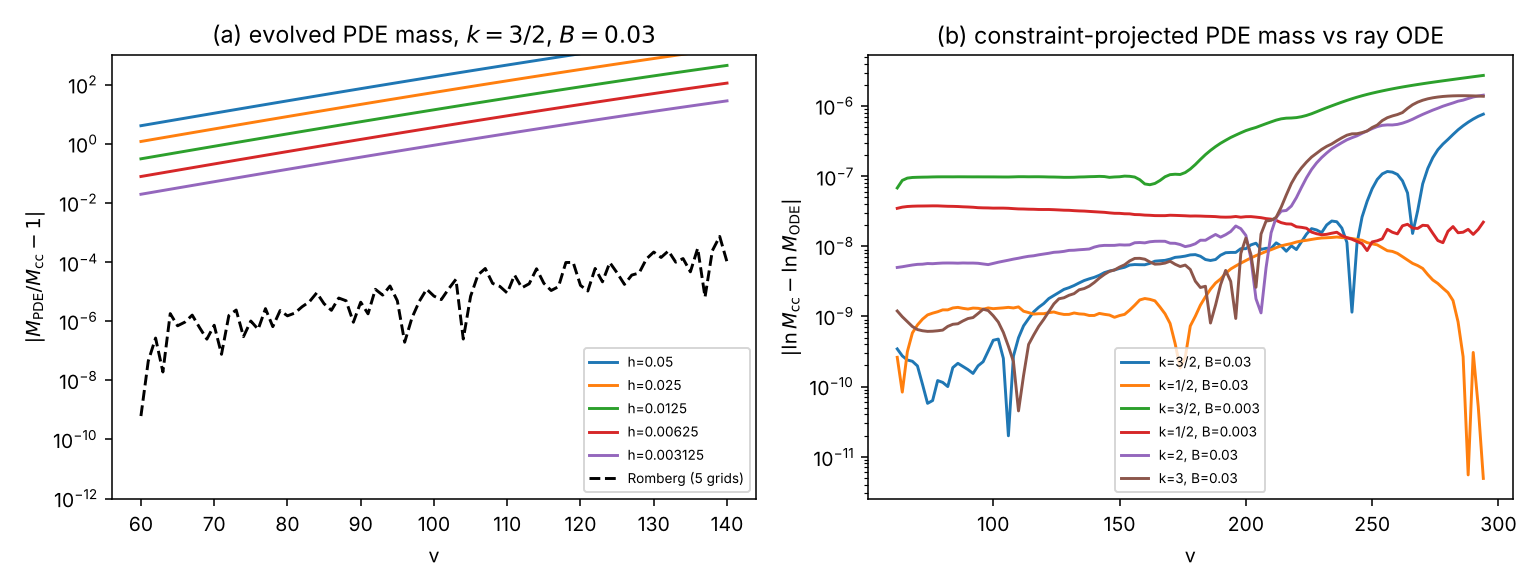
\includegraphics[width=\textwidth]{fig_e13.png}
\caption{Constraint-projected PDE mass. (a) Relative difference of the evolved PDE mass of each grid and of the five-grid extrapolation from $M_{\rm cc}$ ($k=3/2$, $B=0.03$, $U\simeq1$): the single-grid curves scale as $h^2$ and exceed $100\%$ near $v\approx100$ (first grid) to beyond $v=140$. (b) $|\ln M_{\rm cc}-\ln M_{\rm ODE}|$ for the runs of Table~\ref{tab:proj}.}
\label{fig:e13}
\end{figure}

\paragraph{Result.} For the six runs the projected mass and the ray ODE agree to $3.3\times10^{-7}$ ($B=0.03$, $k=3/2$), $1.4\times10^{-8}$ ($k=1/2$), $1.1\times10^{-6}$ ($k=2$), $1.4\times10^{-6}$ ($k=3$), $2.3\times10^{-6}$ ($B=0.003$, $k=3/2$) and $3.7\times10^{-8}$ ($k=1/2$) in $\ln M$ over $84\le v\le280$, i.e.\ over a growth of $M$ by $e^{158}$ to $e^{179}$ ($10^{69}$--$10^{78}$), whereas the extrapolated evolved PDE mass is wrong by $7\times10^{-2}$ at $v=290$ ($B=0.03$, $k=3/2$) and negative at $v=200$ for $B=0.003$. The projected mass itself is stable under the choice of grids: dropping the coarsest grid changes $\ln M_{\rm cc}$ by at most $1.2\times10^{-8}$, $3.6\times10^{-10}$, $1.1\times10^{-7}$, $7.8\times10^{-7}$, $4.5\times10^{-9}$ and $1.3\times10^{-10}$ in the six runs (same order); for $k=3$ it is comparable to the disagreement with the ODE, so there the projected mass is known to about $10^{-6}$ only. The residual disagreement with the ODE is larger than that and grows slowly with $v$ ($\le10^{-7}$ for $v\le160$, $2.3\times10^{-6}$ at $v=280$ for $B=0.003$, $k=3/2$). It is what an error of the extrapolated metric exponent of $\delta\sigma_v\approx1.5\times10^{-9}$ ($B=0.03$) or $10^{-8}$ ($B=0.003$) would produce in the ODE, $d\ln y/dv=\rho/r-\sigma_v+S/y$, integrated over $220$ units, and $M_{\rm cc}$ does not integrate $\sigma_v$ (it enters through $\rho$ only, which is a filtered quantity); these are below or at the level spread of $\sigma_v$ ($1.2\times10^{-8}$, Section~\ref{sec:ray}). We take the projected value as the reference and the disagreement as a bound on the error of $\ln M_{\rm ODE}$ from this source. On the ray $U=0.3$, where $M(v_0)\approx r/2$ and $y$ is close to the unstable point, the ray ODE calibrated on the evolved $y$ is off by $7.6\times10^{-4}$ in $\ln M$ ($B=0.003$, $k=3/2$; $1.1\times10^{-5}$ at $B=0.03$) because the $10^{-9}$ error of the extrapolated $y(v_0)$ is amplified by $e^{\kappa_-\Delta v}$ before $y$ leaves the neighbourhood of $\tfrac12$; the projected mass has no such sensitivity, since it needs no $y(v_0)$.

What the projected mass does not do: it takes the same extrapolated $\sigma_v$ and $\phi_v$ (through $\rho$) as the ODE, so it does not reduce their uncertainty: for $k=1/2$ at $B=0.03$ the excess of $|\sigma_v|$ over $\kappa_-(\mu_f)$, extrapolated beyond $v=250$ in the kernel-driven extension, remains the dominant uncertainty of $\ln M$ there. It is a reference for the PDE solution, not for the equations.

\paragraph{The tail exponent in $M$.} Table~\ref{tab:ray} and Figure~\ref{fig:ray} show $q_M$. For $k=3/2$ it rises to $11.2$ at $v=140$, falls through $5.99$ at $v=260$ and reaches $5.51$ at $v=290$: the overshoot and the return to $2k+2=5$ are those of the flux exponent (Table~\ref{tab:long}), now seen in $M$ and not in $\phi_v$ alone. For $k=1/2$ it passes through $3.79$ at $v=84$ and reaches $2.83$ at $v=290$, approaching $3$ from below because $|\sigma_v|$ has not relaxed to $\kappa_-(\mu_f)$ (the excess is $1.1\times10^{-3}$ at $v=290$, which contributes $-(|\sigma_v|-\kappa_-)(v+1)=-0.32$).

\begin{figure}[t]
\centering
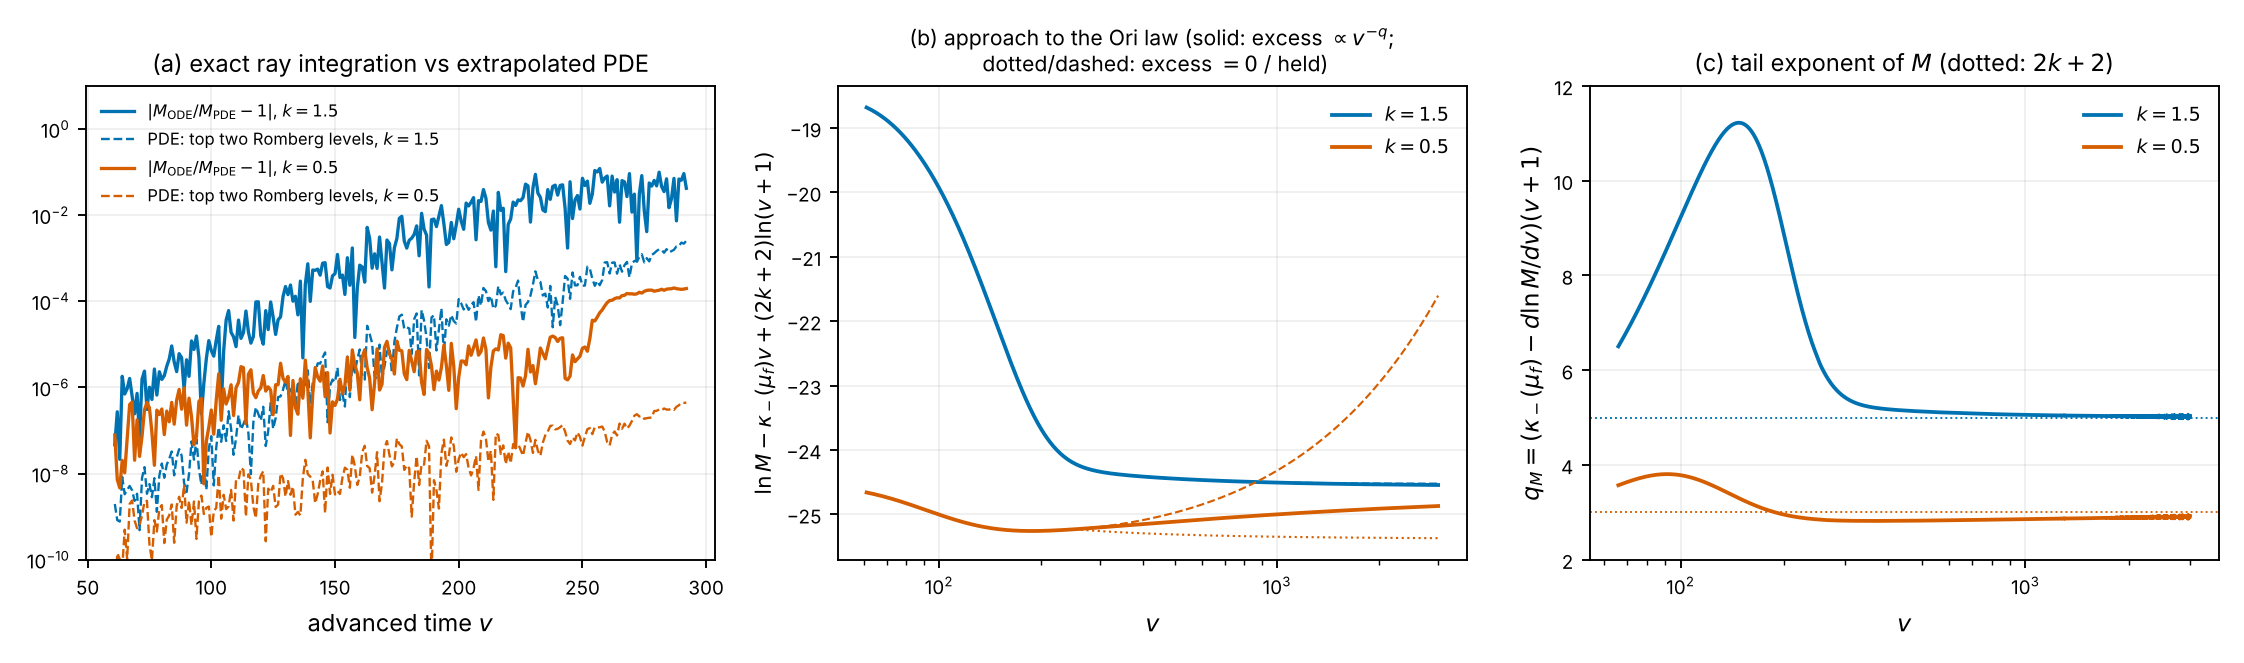
\includegraphics[width=\textwidth]{fig_ray_mass.png}
\caption{Exact ray integration of $M$ ($B=0.03$, $U=1$, $v_0=60$). (a) $|M_{\rm ODE}/M_{\rm PDE}-1|$ (solid) and the spread of the two highest Romberg levels of $M_{\rm PDE}$ (dashed). The solid curve lies above the dashed one by $10^{2}$--$10^{3}$ at every $v$ (see text). For $v>250$ the ODE inputs are kernel-driven, so the $k=1/2$ curve there measures the error of the kernel inputs ($\approx2\times10^{-4}$ in $M$ at $v=290$). (b) $\ln M-\kappa_-(\mu_f)v+(2k+2)\ln(v+1)$ to $v=3000$ with the excess of $|\sigma_v|$ over $\kappa_-(\mu_f)$ decaying as a fitted power (solid), set to zero (dotted) or held (dashed) beyond $v=250$. (c) $q_M$ (dotted: $2k+2$).}
\label{fig:ray}
\end{figure}

\paragraph{Kernel-driven extension to $v=3000$.} The PDE inputs are available to $v=300$. Beyond $v_b=250$ we use $\phi_v=r_b\,(K*j)$ with the interior kernel of Section~\ref{sec:kernel-deriv} (no fitted parameter; $r_b=1.035$ is the PDE-to-kernel flux ratio at $v_b$ for $B=0.03$, held constant: the nonlinear $3.5\%$ of Section~\ref{sec:kernel-tests}(d), which changes by $\le10^{-3}$ between $v=250$ and $290$ and which, with the kernel of the final hole ($r_b=1.0067$, $1.0188$, $1.0058$, $1.0055$ for $k=3/2$, $1/2$, $2$, $3$; constant in $v$), changes the results below by $\le0.05$ in $\ln M$ at $v=2500$) and $|\sigma_v|=\kappa_-(\mu_f)+e(v)$, with $e(v)$ the measured excess at $v_b$ ($1.4\times10^{-3}$ for $k=1/2$ and $8.3\times10^{-6}$ for $k=3/2$) continued as $e(v_b)(v_b/v)^{q}$, $q=1.48$ and $4.42$ fitted on $150\le v\le250$; bounds are $e=0$ and $e=e(v_b)$ held. We integrate \eqref{eq:ray} in $\ln y$ and $\ln\rho$ (\texttt{ray\_extend.py}; the kernel helper is \texttt{kernel\_lib.py}). The PDE-driven and kernel-driven masses can be compared where both exist: at $v=290$ they differ by $1.5\times10^{-3}$ ($k=3/2$, $B=0.03$; $\ln M=174.908$ against $174.906$) and by $2\times10^{-4}$ ($k=1/2$). Results:
\begin{center}\small
\begin{tabular}{rcccc}
\toprule
$v$ & $\ln M$ ($k=3/2$) & $q_M$ ($k=3/2$) & $\ln M$ ($k=1/2$) & $q_M$ ($k=1/2$)\\
\midrule
290 & 174.91 & 5.51 & 186.67 & 2.83\\
400 & 259.55 & 5.175 & 272.59 & 2.82\\
1000 & 725.77 & 5.058 & 743.57 & 2.86\\
2000 & 1507.10 & 5.028 & 1530.87 & 2.89\\
2500 & 1898.39 & 5.022 & 1924.88 & 2.90\\
\bottomrule
\end{tabular}
\end{center}
For $k=3/2$, $q_M=5.02$ at $v=2500$ against $2k+2=5$ and $\ln M-\kappa_-(\mu_f)v+5\ln(v+1)$ is $-24.541$ at $v=2500$ and changes by $5\times10^{-3}$ between $2000$ and $2500$: the Ori law $M\propto v^{-(2k+2)}e^{\kappa_-(\mu_f)v}$ is reached in $M$ at $v\gtrsim10^3$, the prefactor being set by the history. The three treatments of the excess differ by at most $0.02$ in $\ln M$ ($k=3/2$, $v=2500$). For $k=1/2$ at $B=0.03$ the corresponding quantity is not converged: $q_M$ is still rising ($2.90$ at $v=2500$) and the three treatments of the excess change $\ln M$ by $-0.48$, $+2.6$ at $v=2500$ (out of $1925$), so the prefactor is uncertain at that level and the approach to $3$ is an extrapolation in the excess; the rate itself changes by at most $10^{-3}$. A rate-only version, with $r$ and $|\sigma_v|$ constant and the kernel flux, gives $q_M(v=3000)=3.012,\,5.019,\,6.023,\,8.030$ for $k=1/2,\,3/2,\,2,\,3$ (\texttt{ray\_rate\_only.py}), with the 10\% crossover of the flux at $v=197,\,309,\,368,\,495$ (Section~\ref{sec:kernel-long}); this is a statement about the filtering of the kernel flux and is independent of the PDE.

\paragraph{Smaller amplitude, $B=0.003$.} The same runs at $B=0.003$ ($\mu_f=5.9\times10^{-5}$ and $9.9\times10^{-5}$) show where the extrapolated mass fails. For $k=1/2$ the ray integration agrees with $M_{\rm PDE}$ to $4.8\times10^{-4}$ for $v\le108$ and to $8.5\times10^{-4}$ at $v=240$. For $k=3/2$ it differs by $1.0\times10^{-2}$ at $v=100$ (two highest Romberg levels: $5\times10^{-6}$), by $-0.19$ at $v=180$, and $M_{\rm PDE}<0$ at $v=200$. The extrapolated mass is less accurate at the smaller amplitude (differences from the ray integration at $v=100$: $5\times10^{-5}$ and $10^{-2}$ for $k=1/2$, $3/2$, against $3\times10^{-7}$ and $7\times10^{-6}$ at $B=0.03$), as expected if the truncation noise does not shrink with $B$ while the mass does ($M(v=108)$ is $1.2\times10^{4}$ and $5\times10^{3}$ times smaller at $B=0.003$), and its level spread does not warn of it; the scaling $C_y\propto B^{-2}$ found above supports this for $y$. The ray equations are unaffected: the ODE rate agrees with $4\pi r\phi_v^2/\rho$ and with $\lambda-\lambda'/\lambda$ to $5\times10^{-6}$ ($k=3/2$, $v=290$; $2\times10^{-5}$ at $v=140$), and the excess $|\sigma_v|-\kappa_-(\mu_f)$ is only $1.1\times10^{-5}$ and $5\times10^{-8}$ at $v=290$, so the extension to $v=3000$ no longer depends on its treatment. It gives $q_M=3.145$ at $v=290$ and $3.012$ at $v=2500$ for $k=1/2$, and $5.509$, $5.022$ for $k=3/2$, i.e.\ $2k+2$ from above for both tails; $\ln M-\kappa_-(\mu_f)v+(2k+2)\ln(v+1)$ changes by $3\times10^{-3}$ and $6\times10^{-3}$ between $v=2000$ and $2500$, and the three treatments of the excess change $\ln M$ by at most $0.025$ out of $1930$ (\texttt{results\_ray\_extend\_B0.003\_k*.txt}).

\paragraph{Physical tails ($k=2,3$).} The tails expected from Price's law on $\mathcal H^+$ (Section~\ref{sec:kernel-long}) were run at $B=0.03$ to $v_1=300$ on the same five grids ($\mu_f=1.070\times10^{-2}$ and $1.154\times10^{-2}$, $\kappa_-(\mu_f)=0.783979$ and $0.783028$). The constraint-projected mass agrees with the ray integration to $1.1\times10^{-6}$ and $1.4\times10^{-6}$ in $\ln M$ up to $v=280$ (Table~\ref{tab:proj}), with growth of $M$ by $e^{162}$ and $e^{158}$. The excess of $|\sigma_v|$ over $\kappa_-(\mu_f)$ at $v_b=250$ is only $9.6\times10^{-7}$ and $3.1\times10^{-7}$, so the extension does not depend on its treatment (the three treatments differ by at most $2.1\times10^{-3}$ and $6.9\times10^{-4}$ in $\ln M$ at $v=2500$). The matching factor of the kernel flux at $v_b$ is $1.0440$ and $1.0639$ for the kernel of the static hole and drifts by $0.6\%$ and $0.3\%$ between $v=250$ and $290$, but is $1.0058$ and $1.0055$ and constant for the kernel of the final hole (Section~\ref{sec:kernel-tests}(d)); with the latter the kernel-driven and PDE-driven $\ln M$ agree at $v=290$ to $10^{-3}$ for all four runs at $B=0.03$ (with the static kernel they differ by $1.0\times10^{-2}$, $-5.6\times10^{-3}$, $1.7\times10^{-3}$ and $5.8\times10^{-4}$ for $k=2,\,3,\,3/2,\,1/2$, i.e.\ twice the drift of the factor). The kernel-driven mass gives $q_M=6.026$ ($k=2$) and $8.035$ ($k=3$) at $v=2500$ against $2k+2=6$ and $8$, from above as for the other tails, and $\ln M-\kappa_-(\mu_f)v+(2k+2)\ln(v+1)=-24.112$ and $-23.332$ there (changes of $7\times10^{-3}$ and $9\times10^{-3}$ since $v=2000$). Before the power law is established the rate is lower and $q_M$ is large: at $v=290$ the rate is $0.7540$ ($k=2$) and $0.6882$ ($k=3$), $q_M=8.73$ and $27.6$, and at $v=400$ $q_M=6.27$ and $16.8$: the flux of the steep tails is still dominated by the memory component at these $v$ (the kernel puts the crossover at $v\approx370$ and $500$), and the PDE reaches $v=300$ only. The statement that $M$ reaches the Ori tail law for these tails therefore rests on the kernel-driven extension beyond $v_b$ (to $10^{-3}$ in $\ln M$ where it can be compared with the PDE, $v\le298$), as for the other tails.

\paragraph{Physical tails at $B=0.003$.} The same two tails at $B=0.003$ ($\mu_f=1.068\times10^{-4}$ and $1.151\times10^{-4}$, $\kappa_-(\mu_f)=0.795537$ and $0.795528$; \texttt{gen3\_B0.003\_k2\_v300.json}, \texttt{gen3\_B0.003\_k3\_v300.json}) give, on the ray $U\simeq1$, a disagreement between the constraint-projected mass and the ray ODE of $2.3\times10^{-6}$ and $5.4\times10^{-7}$ in $\ln M$ at $v=280$ (growth of $M$ by $e^{156}$ and $e^{152}$; $\le10^{-6}$ for $84\le v\le200$), and on the ray $U=0.3$ of $8.7\times10^{-4}$ and $9.6\times10^{-4}$, the calibration amplification described above (\texttt{results\_e13\_B0.003\_k2.txt}, \texttt{k3}). The flux is reproduced by the kernel of the final hole to $0.99993$ and $0.99947$ at $v=280$, i.e.\ within the linear-order accuracy of the kernel at this amplitude ($\le5\times10^{-4}$, Section~\ref{sec:kernel-tests}), so the matching factor at $v_b$ is $0.99982$ and $0.99947$ against $1.0058$ and $1.0055$ at $B=0.03$: the difference is the $B^2$ remainder of Section~\ref{sec:kernel-tests}(d). The excess of $|\sigma_v|$ over $\kappa_-(\mu_f)$ at $v_b=250$ is $9\times10^{-9}$ and $3\times10^{-9}$, below the level spread of $\sigma_v$, and the three treatments of it differ by at most $2\times10^{-5}$ and $7\times10^{-6}$ in $\ln M$ at $v=2500$. The kernel-driven mass gives $q_M=6.0261$ and $8.0352$ at $v=2500$, equal to the $B=0.03$ values ($6.026$, $8.035$) to the printed digits, and $\ln M-\kappa_-(\mu_f)v+(2k+2)\ln(v+1)=-33.834$ and $-33.104$ there (changes of $6.6\times10^{-3}$ and $8.9\times10^{-3}$ since $v=2000$). The approach of $q_M$ to $2k+2$ from above, and the value reached at $v=2500$, are therefore independent of the amplitude for the physical tails, as the rate-only calculation implies; and the indicators of the curvature section of Paper~E are converged at this amplitude (extendibility table of Paper~E, last two rows).

\paragraph{Caveats.} (i) The ray equations are consequences of the field equations: this subsection tests the numerical solution up to $v=290$ and extends it by the model beyond, and it is not an independent derivation of the amplitude of $M$. (ii) The ray ODE is calibrated with $r,\rho,y$ at $v_0$ from the PDE. The constraint-projected mass removes the calibration of $y$ and confirms the ODE (Table~\ref{tab:proj}); the amplitude of $M$ remains that of the discrete solution, through the extrapolated $\sigma_v,\phi_v$, the profile integral and $r,\rho$ at $v_0$. The evolved $y$ is meaningful only where the physical $y$ exceeds the truncation noise: for the static interior ($B=0$, $y=1/2$ exactly) the single-grid $y$ on $U=1$ is $-0.8,\,-3.7\times10^{3},\,-1.1\times10^{7}$ at $v=40,50,60$ on the coarsest grid and the three-grid Romberg value is wrong by $7$ at $v=60$ (\texttt{results\_static\_y\_noise.txt}); for the tail data $y$ at $v_0=60$ is dominated by the physical mass. The starting points $v_0=48,\dots,84$ give the same curve, which supports the calibration. At $B=0.003$, $k=3/2$, $M(v_0=60)=0.85$ is marginal. (iii) Beyond $v=250$ the inputs are the kernel flux (linear response of a static interior, matched at $v_b$ by a constant factor, no back-reaction of the accumulated mass on $\kappa_-$ beyond the measured excess) and an extrapolated excess of $|\sigma_v|$; for $k=1/2$ at $B=0.03$ this matters (above). The approach of $q_M$ to $2k+2$ is a property of this model: filtering a power-law flux with the rate $\kappa_-$ gives it for any inputs (the rate-only runs have no PDE input). (iv) The closure is additive, one tail amplitude and one inner profile. (v) $M$ is the Misner--Sharp mass on a ray $U=1$ at $r\approx1.06$, not the mass of the shell model; the agreement of the two rates is that of Section~\ref{sec:kernel-shell}.


\section{What the method settles, and what it does not}
\label{sec:limits}

\paragraph{What it settles.} In the additive-closure system, with data regular on the event horizon: (i) the metric exponent follows $\kappa_-(\mu_f)$ and not the static value (Section~\ref{sec:ehdata}); (ii) the Cauchy-horizon flux is the linear response of the static interior to the horizon flux, its kernel and decay rate $\kappa_+$ follow from the interior wave equation and it is confirmed by the evolution to $4\times10^{-4}$ ($B=0.003$; to $v=420$ for $k=3/2$ at $3\times10^{-4}$, constant to $2\times10^{-5}$), and the part of the excess at $B=0.03$ that is not the displacement of the horizons is intrinsic second order and has no universal coefficient (Section~\ref{sec:kernel}); (iii) along a ray the field equations give the mass without the evolved first derivatives, and this reproduces the extrapolated PDE mass to $6\times10^{-5}$ ($k=3/2$) and $2\times10^{-6}$ ($k=1/2$) to $v=108$, while the constraint-projected PDE mass agrees with it to $10^{-6}$ in $\ln M$ to $v=280$ (Section~\ref{sec:ray}); (iv) with a kernel-driven flux beyond $v=250$ the tail law $2k+2$ is reached in $M$ at $v\gtrsim10^{3}$, and in the window the PDE reaches the rate is $\kappa_-(\mu_f)-2\kappa_+$ for steep tails, not the tail law.

\paragraph{Limits.}
\begin{enumerate}
\item \emph{Closure.} The system is the additive closure. The static sector of the mass-tracking closure of the series is realised in four-dimensional quasi-topological gravity, whose double-null dynamics is the subject of Paper~F; the ingredients of the pipeline (event-horizon-regular data from the exact static solution and the teleological horizon, linear-kernel comparison of the flux, the metric exponent) are applied to it in Paper~F with a constrained evolution that integrates the two Raychaudhuri equations; there the flux through the interior agrees with the kernel of this paper to $8\times10^{-4}$ and differs from the additive closure by terms $\propto B^{2}$. The exact ray integration and the constraint-projected mass are not carried over to that system, and its evolution does not reach the tail regime.
\item \emph{Range.} The nonlinear runs reach $v=110$ at $\kappa_-v\approx87$ (to $v=300$ for the flux and the metric exponent, to $v=440$ for the flux at $B=0.003$, $k=3/2$), not $v=\infty$; the mass is reconstructed to $v=290$ by the ray integration, confirmed to $v=280$ by the constraint-projected mass, and extended to $v=3000$ by a model.
\item \emph{Rate of the metric exponent.} For $k=1/2$ at $B\ge0.03$ the excess of $|\sigma_v|$ over $\kappa_-(\mu_f)$ is not relaxed within $v\le300$ and enters the extension as an extrapolated quantity; for $k=3/2$ it is $\le10^{-5}$.
\item \emph{Flux beyond $v\approx250$ at $B=0.03$.} It is the kernel prediction with a constant matching factor of the final-hole kernel; the factor is constant in $v$ to $10^{-3}$ in $250\le v\le290$ and the choice of kernel changes $\ln M(v=2500)$ by $\le0.05$, but it is not independently measured there. At $B=0.003$, $k=3/2$ the kernel is confirmed by the PDE to $v=420$ (Section~\ref{sec:kernel-tests}(e)), with the caveat there that the error control of $\phi_v$ beyond $v\approx300$ is weaker than that of $M$.
\item \emph{Amplitude of $M$.} The ray equations are consequences of the field equations: this tests the numerical solution, it is not an independent derivation of the amplitude of $M$, which is that of the discrete solution through $\sigma_v$, $\phi_v$, the profile integral and $r,\rho$ at $v_0$.
\item \emph{Parameters.} One inner profile ($m_N=5$, $a_N=10$) for the nonlinear runs; two tail amplitudes for the five main series and, for the long runs, $B=0.003$; four seeds, of which two give a clean result and one is non-perturbative; the Richardson--Romberg extrapolation assumes an expansion in $h^{2}$ (checked by the internal convergence, the differential relation, the exact ray integration and the constraint-projected mass).
\item \emph{Second-order remainder.} Its coefficient is not computed: second-order perturbation theory of the scalar equation on the dynamical background is needed.
\end{enumerate}

\section*{Reproducibility}
\raggedright
The event-horizon runs of Section~\ref{sec:ehdata} are in \texttt{paperE\_inner\_horizon/code/eh\_init/} of the bundle: \texttt{dnU.py} (exact static solution in $(U,v)$, teleological horizon data, grid map, constraint-consistent seed); \texttt{run\_tail.py}, \texttt{t\_static4.py}, \texttt{conv1.py}, \texttt{mucheck.py}, \texttt{nanloc.py}, \texttt{muid.py}, \texttt{seed5.py}, \texttt{diffrate5.py}, \texttt{phiexp.py}, \texttt{phiexp\_extrap.py}, \texttt{conv3.py}, \texttt{noise.py}, \texttt{t\_uniform.py}; the five-grid pipeline \texttt{stream.c} (two-row streaming copy of the evolution routine), \texttt{gen.py} (one run per data set, writes the JSON), \texttt{analyze.py} (Romberg extrapolation of the signed series, absolute values taken afterwards; rate against $\lambda$), \texttt{report\_stream.py} (the numbers of Table~\ref{tab:ehrate} and the $\phi_v$ exponents), \texttt{aniso.py}, \texttt{check\_field\_equations.py} (Eqs.~\eqref{eq:dn1}--\eqref{eq:dn3} and the Kretschmann decomposition); the kernel of Section~\ref{sec:kernel}: \texttt{transfer.py}, \texttt{transfer\_vec.py}, \texttt{residues.py}, \texttt{trace\_residues.py}, \texttt{kernel\_ft2.py}, \texttt{kernel\_analytic.py}, \texttt{kernel\_general.py}, \texttt{kernel\_mN.py}, \texttt{crossover\_analytic.py}, \texttt{shell\_kernel.py}, \texttt{flux\_nl.py}, \texttt{longrun.py}, \texttt{kernel\_vs\_long.py}, \texttt{kernel\_test.py}, \texttt{phidecay.py}; the exact mass integration of Section~\ref{sec:ray}: \texttt{gen2.py} (stores $M$ and all eight fields per ray and grid), \texttt{raylib.py} (Eq.~\eqref{eq:ray}), \texttt{ray\_validate.py}, \texttt{ray\_long.py}, \texttt{ray\_mass.py} (Table~\ref{tab:ray}), \texttt{kernel\_lib.py}, \texttt{ray\_extend.py} (kernel-driven extension), \texttt{ray\_rate\_only.py}, \texttt{ray\_fig.py}; the PDE reference of the same section: \texttt{stream2.c} (streaming evolution that also accumulates the row integral of Eq.~\eqref{eq:yc}), \texttt{gen3.py}, \texttt{e13\_project.py}, \texttt{e13\_all.py}, \texttt{e13\_errconst.py}, \texttt{e13\_table.py}, \texttt{e13\_fig.py}; the matching factor: \texttt{transfer\_mu.py}, \texttt{transfer\_vec\_mu.py}, \texttt{kernel\_mu.py}, \texttt{kernel\_lib\_mu.py}, \texttt{e11\_ratio.py}, \texttt{e11\_scaling.py}, \texttt{e11\_pulse.py}; the flux to $v=420$: \texttt{e12\_ratio.py} (\texttt{results\_e12\_ratio.txt}, data \texttt{gen3\_B0.003\_k1.5\_v450.json}); the JSON files \texttt{gen\_*.json}, \texttt{gen2\_*.json}, \texttt{gen3\_*.json}; logs in \texttt{results\_*.txt}; \texttt{dn2lib.py} is the Python wrapper of the evolution routine, which is the unchanged \texttt{double\_null.c} of \texttt{paperE\_inner\_horizon/code/nonlinear/}.

\bibliographystyle{plainnat}
\bibliography{references}
\end{document}
